\documentclass[english,11pt]{beamer}

\DeclareMathOperator{\Cov}{Cov}
\DeclareMathOperator{\Var}{Var}
\DeclareMathOperator{\E}{\mathbb{E}}
\DeclareMathOperator{\Proba}{\mathbb{P}}

\newcommand{\Covb}[2]{\ensuremath{\Cov\!\left[#1,#2\right]}}
\newcommand{\Eb}[1]{\ensuremath{\E\!\left[#1\right]}}
\newcommand{\Pb}[1]{\ensuremath{\Proba\!\left[#1\right]}}
\newcommand{\Varb}[1]{\ensuremath{\Var\!\left[#1\right]}}

% norm
\newcommand{\norm}[1]{\| #1 \|}

\newcommand{\indep}{\rotatebox[origin=c]{90}{$\models$}}





\usepackage{mathptmx,amsmath,amssymb,graphicx,bibentry,bbm,babel,ragged2e}

\makeatletter

\newcommand{\noun}[1]{\textsc{#1}}
\newcommand{\jitem}[1]{\item \begin{justify} #1 \end{justify} \vfill{}}
\newcommand{\sframe}[2]{\frame{\frametitle{#1} #2}}

\newenvironment{centercolumns}{\begin{columns}[c]}{\end{columns}}
%\newenvironment{jitem}{\begin{justify}\begin{itemize}}{\end{itemize}\end{justify}}









%\usetheme{Warsaw}
%\setbeamertemplate{footline}[text line]{}
%\setbeamercolor{structure}{fg=purple!50!blue, bg=purple!50!blue}
%\setbeamersize{text margin left=15pt,text margin right=15pt}




\usetheme{Boadilla}


% redefine palette
\definecolor{cybblue}{HTML}{1C6F91}


\setbeamercolor{structure}{fg=cybblue}

\setbeamercovered{transparent}


\addtobeamertemplate{title page}{%\hspace{-0.4cm}
\vspace{-0.8cm}
\hspace{-0.5cm}
%\includegraphics[height=1.2cm,width=1.2\textwidth]{template/bandeau3}\\
}{%
%\begin{textblock*}{150mm}(-1cm,-1.5cm)
%\end{textblock*}
}


\setbeamertemplate{footline}{
\hspace{0.2cm}

\includegraphics[height=0.75cm]{template/medium}
\hfill

\includegraphics[height=0.75cm]{template/eu}
\hspace{0.15cm}
\vspace{0.15cm}
}





\@ifundefined{showcaptionsetup}{}{%
 \PassOptionsToPackage{caption=false}{subfig}}
\usepackage{subfig}

\usepackage[utf8]{inputenc}
\usepackage[T1]{fontenc}


\usepackage[usenames,dvipsnames]{pstricks}
\usepackage{epsfig}



\makeatother

\begin{document}


\title{A Theoretical and Quantitative Geography Insight into Interactions between Networks and Territories}

\author{J.~Raimbault$^{1,2}$\\
\texttt{juste.raimbault@polytechnique.edu}
}


\institute{$^{1}$UMR CNRS 8504 G{\'e}ographie-cit{\'e}s\\
$^{2}$UMR-T IFSTTAR 9403 LVMT\\
}


\date{Seminar - 21th December 2016
}


{


\setbeamertemplate{footline}{
\hspace{0.2cm}

\includegraphics[height=1cm]{template/medium}
\hfill
\textit{This Project is funded by the European Union}\hspace{0.2cm}

\includegraphics[height=1cm]{template/eu}
\hspace{0.2cm}
\vspace{0.5cm}
}


\frame{\maketitle}

}




%%%%%%%%%%%%%%%%%%%
%% ABSTRACT

%Recent advances in Theoretical and Quantitative Geography have witnessed the co-construction of geographical theories, complex models of simulation and Empirical analysis. We build on this legacy to shed light on relations between territories and networks. Our contribution consists in two distincts parts. First we develop a new theory of territorial systems, that emphasizes on the role of networks in co-evolutive processes. More precisely, we speculate, building on several modeling and empirical previous contributions, that within Pumain’s Evolutive Urban Theory [Pumain, 1997], the existence of co-evolutive subsystems is equivalent to the existence of morphogenetic processes in which networks are significant drivers. Implications include the necessity of networks in explaining territorial systems dynamics, but also a modular decomposition of these systems into local stationary processes in space or time.
%In a second part, we discuss practical implications of the theory through the adaptation of a agent- based model introduced in [Le Néchet and Raimbault, 2015], which simulates the co-evolution of land-use and transportation infrastructure within a Mega-city Region. In particular, it includes game theoretical modeling of decision making processes for transportation governance. The model is partially validated on synthetic data by retrieving expected stylized facts on emergent infrastructure. We propose then to apply it to the Mega-city Region of Pearl River Delta, China, which is very typical of included characteristics such as the presence of a strong competition between inner cities and the recent realization, construction or planning of numerous large-scale transportation infrastructures. Calibration of the model will allow first to infer information on potentially hidden governance processes when applied on real or planned infrastructure, and secondly to compare among different possible governance frameworks when applied on hypothetical optimized infrastructure.






%%%%%%%%%%%%%%%%%%%
\section{Introduction}
%%%%%%%%%%%%%%%%%%%


\sframe{Complex Urban Systems}{

\centering

% find typical pictures witnessing a bifurcation in an Urban system. Guangzhou, HK, Zhuhai ?

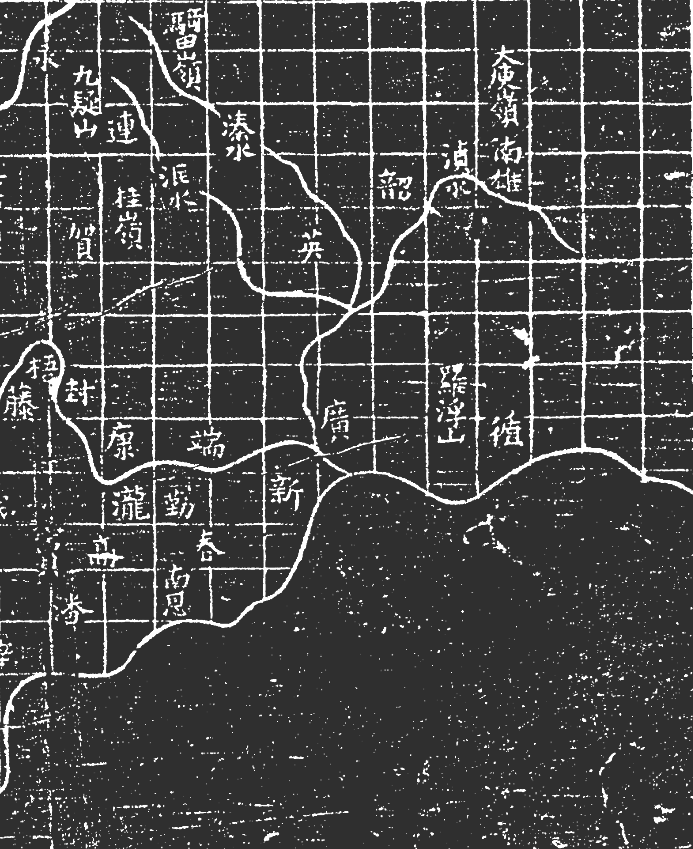
\includegraphics[width=0.3\textwidth,height=0.6\textheight]{figures/Pearl_River_Yujitu}\hspace{0.5cm}
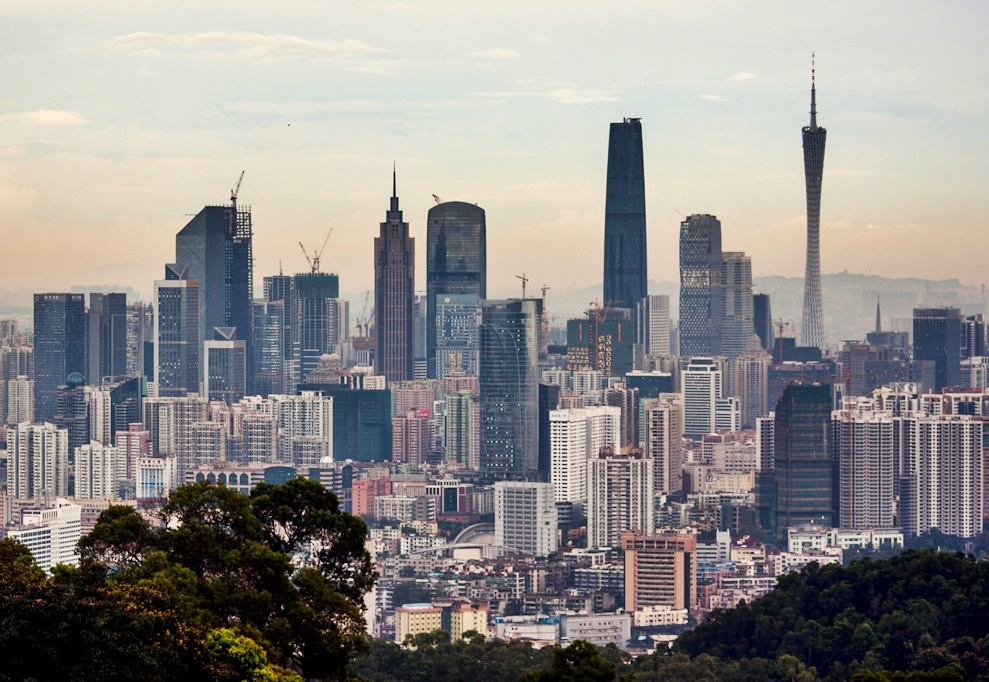
\includegraphics[width=0.5\textwidth,height=0.6\textheight]{figures/Guangzhou_skyline}

{\tiny Source : Wikipedia}

}





%\sframe{Complex Systems Approaches in Science}{
%
%\justify
%% exemples of CS Approaches / emergence 
%% -> why CS ?
%
%$\rightarrow$ Failure of reductionism already highlighted by Anderson in 1972
%
%\cite{anderson1972more}
%
%\medskip
%
%$\rightarrow$ Yet few domains with Integrative Theories : see e.g. Economics
%
%\cite{farmer2009economy}, Urban Science \cite{portugali2012complexity}
%
%\medskip
%
%$\rightarrow$ Even physics begins to realize the potential of this ``New Kind of Science~\cite{wolfram2002new} : Quantum coherence paradox solved through computational complexity~\cite{2014arXiv1403.7686B} ; Very recent theory of emergent gravity solves Dark Matter issue~\cite{2016arXiv161102269V}
%
%\medskip
%
%$\rightarrow$ Towards Complex Systems Sciences aiming at vertical integration (integrative disciplines) and horizontal integration (interdisciplinary transversal problems) : see e.g. CS roadmap \cite{2009arXiv0907.2221B}
%
%
%}


\sframe{Theoretical and Quantitative Geography}{

% adapt Sander's schema (adding methods and tools)
%  Q : each "space" is indeed a dimension , and links are rotations ? not euclidian space.

An extended framework for TQG~\cite{livet2010}

\bigskip

\centering

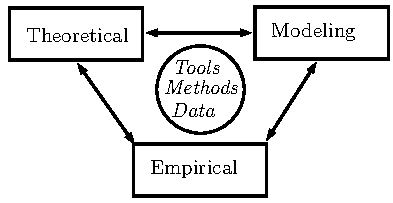
\includegraphics[height=0.5\textheight,width=0.8\textwidth]{figures/tqg.pdf}

\bigskip

\textit{To go further : speculative embedding of this scheme into a meta-modeling framework~\cite{raimbault2016memoire}}


}



\sframe{Complex Urban Systems}{

% slide to explain context of thesis and content here ; otherwise a bit confusing.

\textbf{Research Context : } \textit{Investigate relations between Networks and Territories, in particular through the construction of models of co-evolution between land-use and transportation network, strangely absent in the literature~\cite{raimbault2015models}.}

\bigskip

$\rightarrow$ Collection of evidences from previous research ; proposition of a geographical theory 

\medskip

$\rightarrow$ Application to Transportation Governance Modeling ; potential insights from application to Pearl River Delta

}



%%%%%%%%%%%%%%%%%%%
\section{Towards a Theory}
%%%%%%%%%%%%%%%%%%%




\sframe{Non-equilibrium dynamics in Transportation Systems}{

Investigation of empirical existence of Static User Equilibrium \cite{2016arXiv160805266R} : data collection and empirical analysis for Parisian highway system

\medskip

\begin{columns}
\column{0.45\textwidth}
\centering
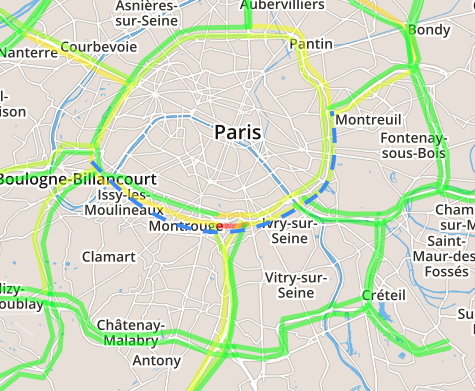
\includegraphics[width=0.65\textwidth]{figures/treq_gr21}\\\medskip
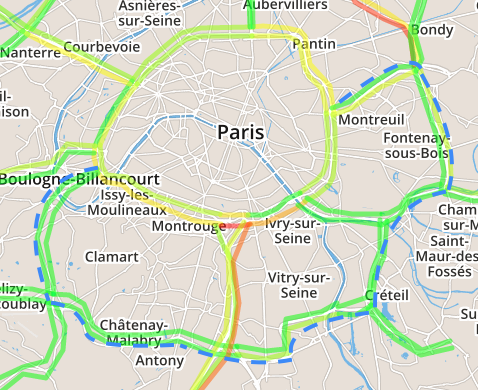
\includegraphics[width=0.65\textwidth]{figures/treq_gr22}

\column{0.55\textwidth}
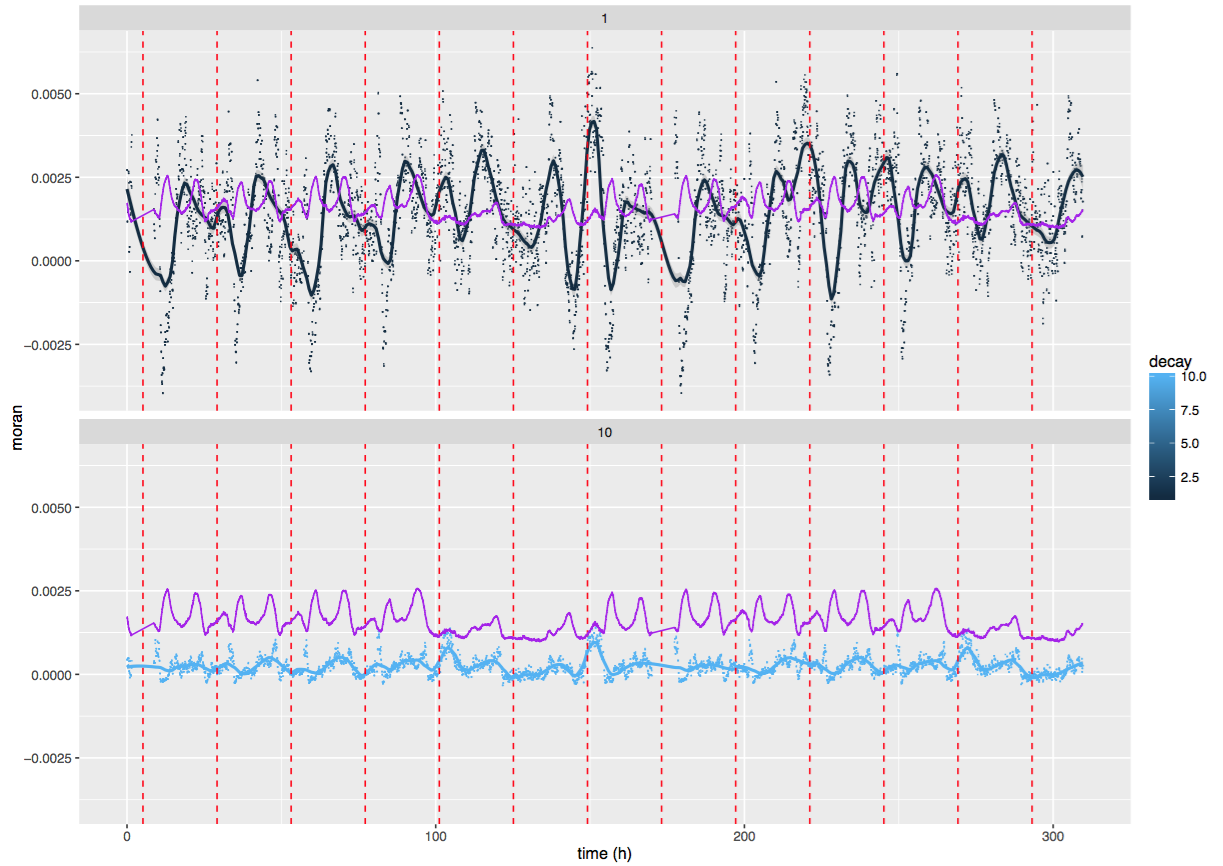
\includegraphics[width=\textwidth]{figures/treq_gr5}

\end{columns}

}

\sframe{Agent-based Modeling of Transportation Systems}{

Agent-based model to investigate user-based policies for a bike-sharing transportation system \cite{raimbault2015user} ; hybrid modeling with statistics and discrete-choice models \cite{raimbault2015hybrid}

\bigskip

\begin{columns}
\column{0.55\textwidth}
\centering
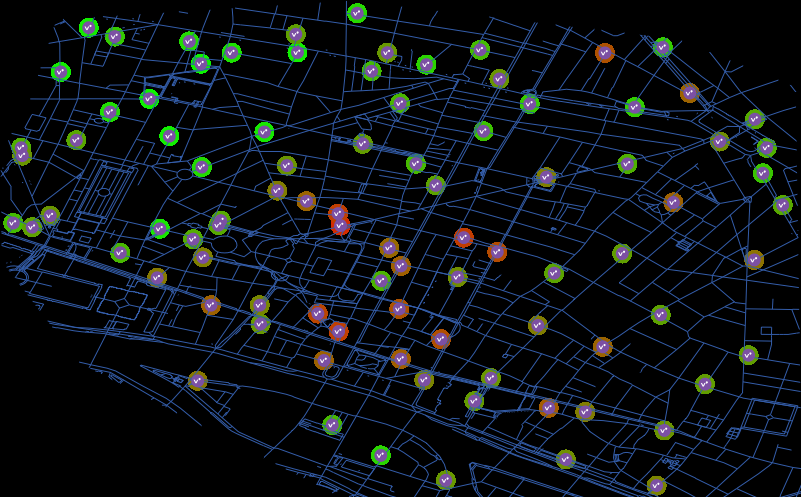
\includegraphics[width=0.9\textwidth]{figures/bikesharing_lfMidday}

\column{0.45\textwidth}
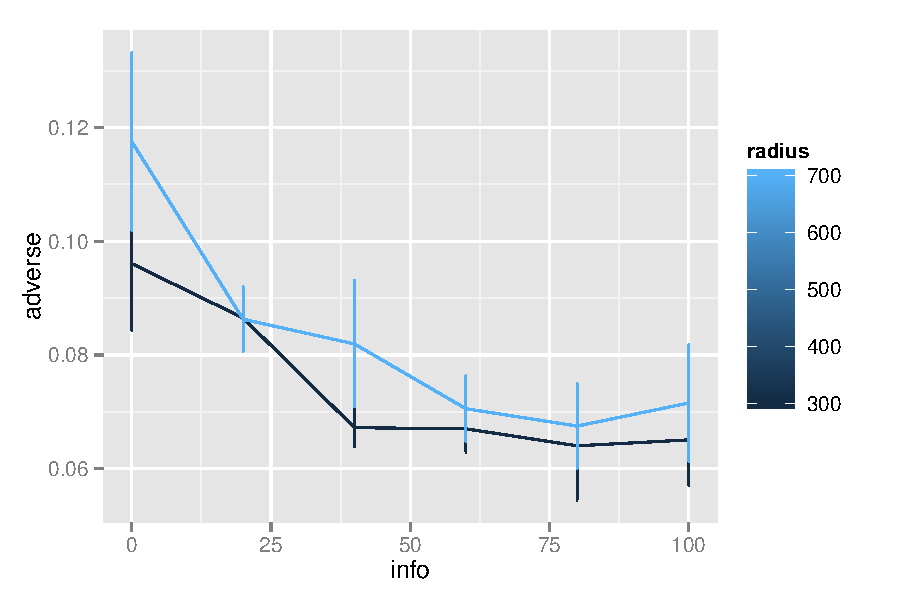
\includegraphics[width=\textwidth]{figures/bikesharing_adverse}

\end{columns}

}


\sframe{Robustness of Multi-attribute Evaluations}{

Data-driven and Model-independant framework to compare robustnesses of multi-attributes evaluations \cite{raimbault2016discrepancy}

\bigskip

\begin{columns}
\column{0.65\textwidth}
\centering
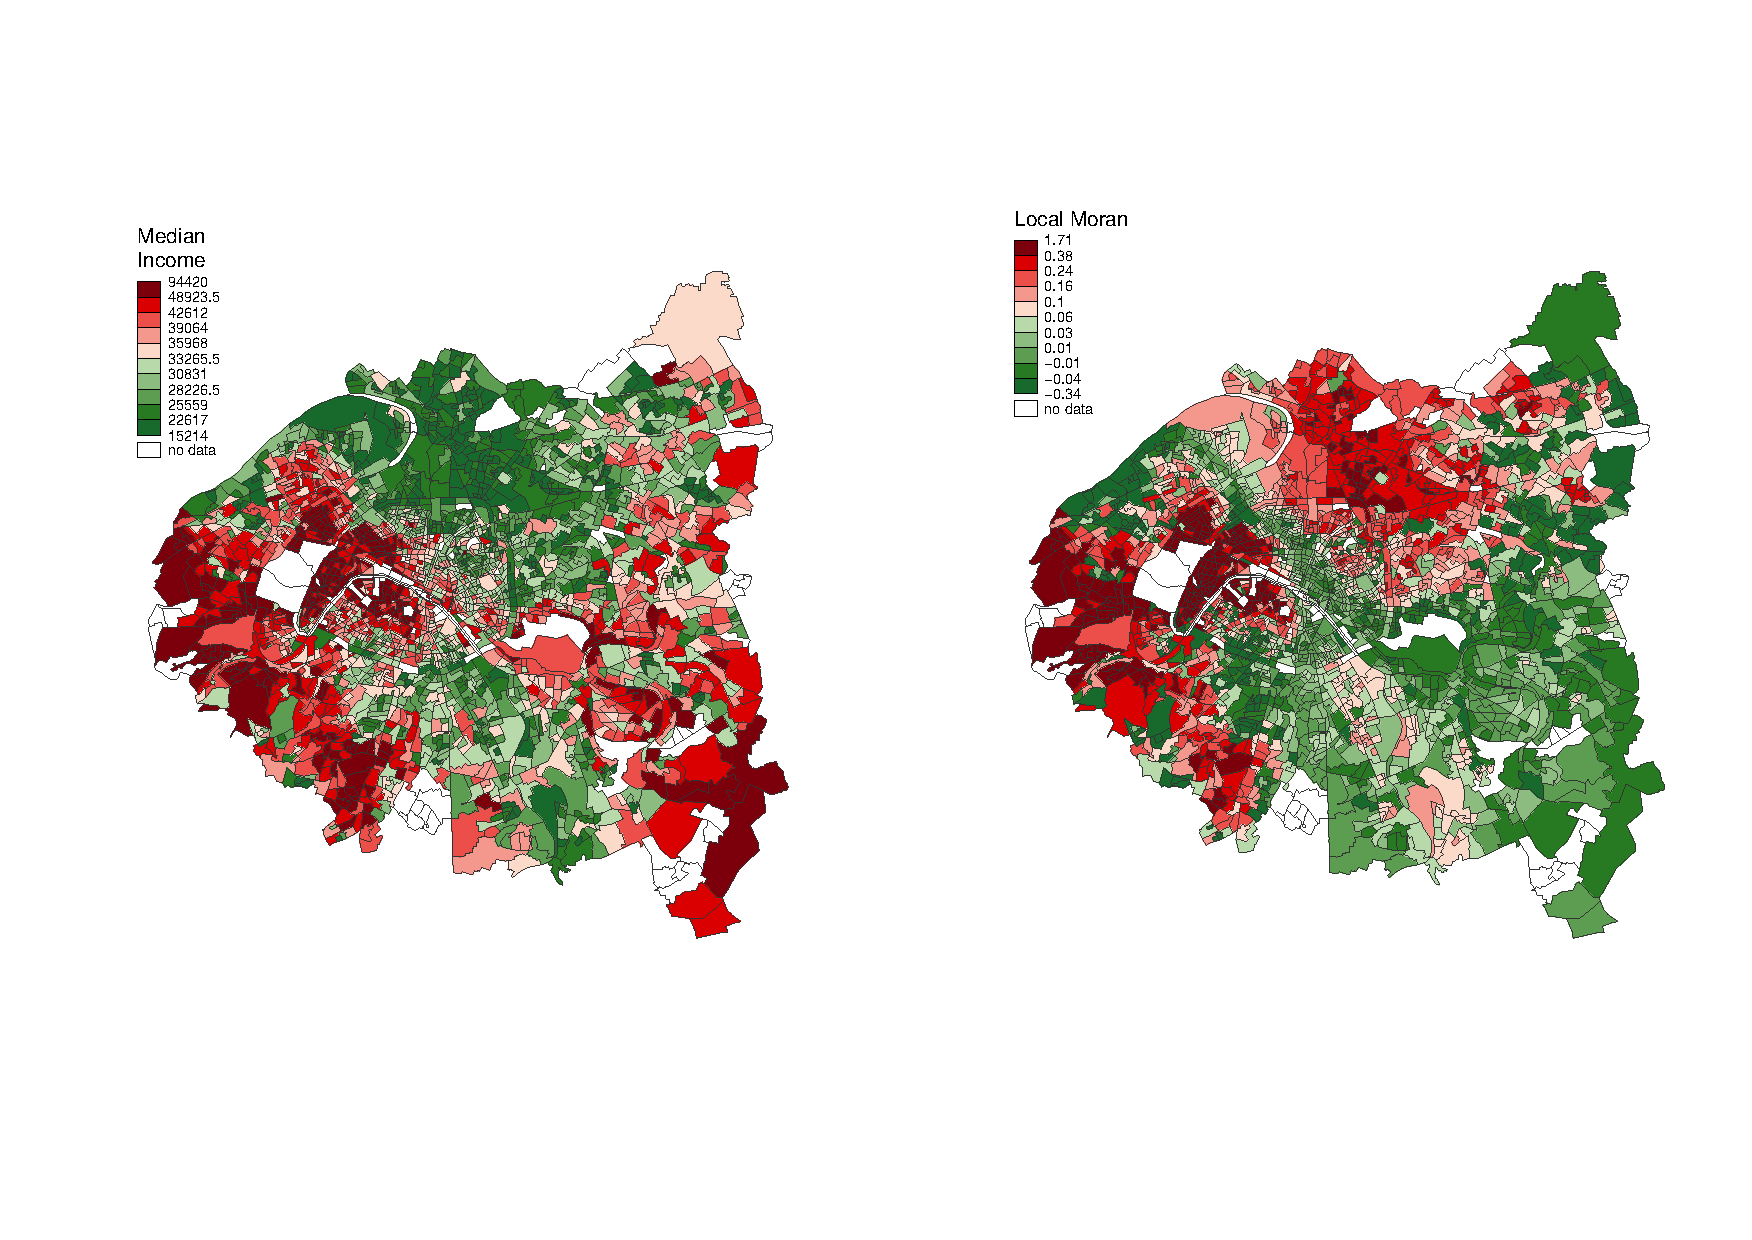
\includegraphics[width=\textwidth]{figures/rob_grandParis_income_moran}

\column{0.35\textwidth}
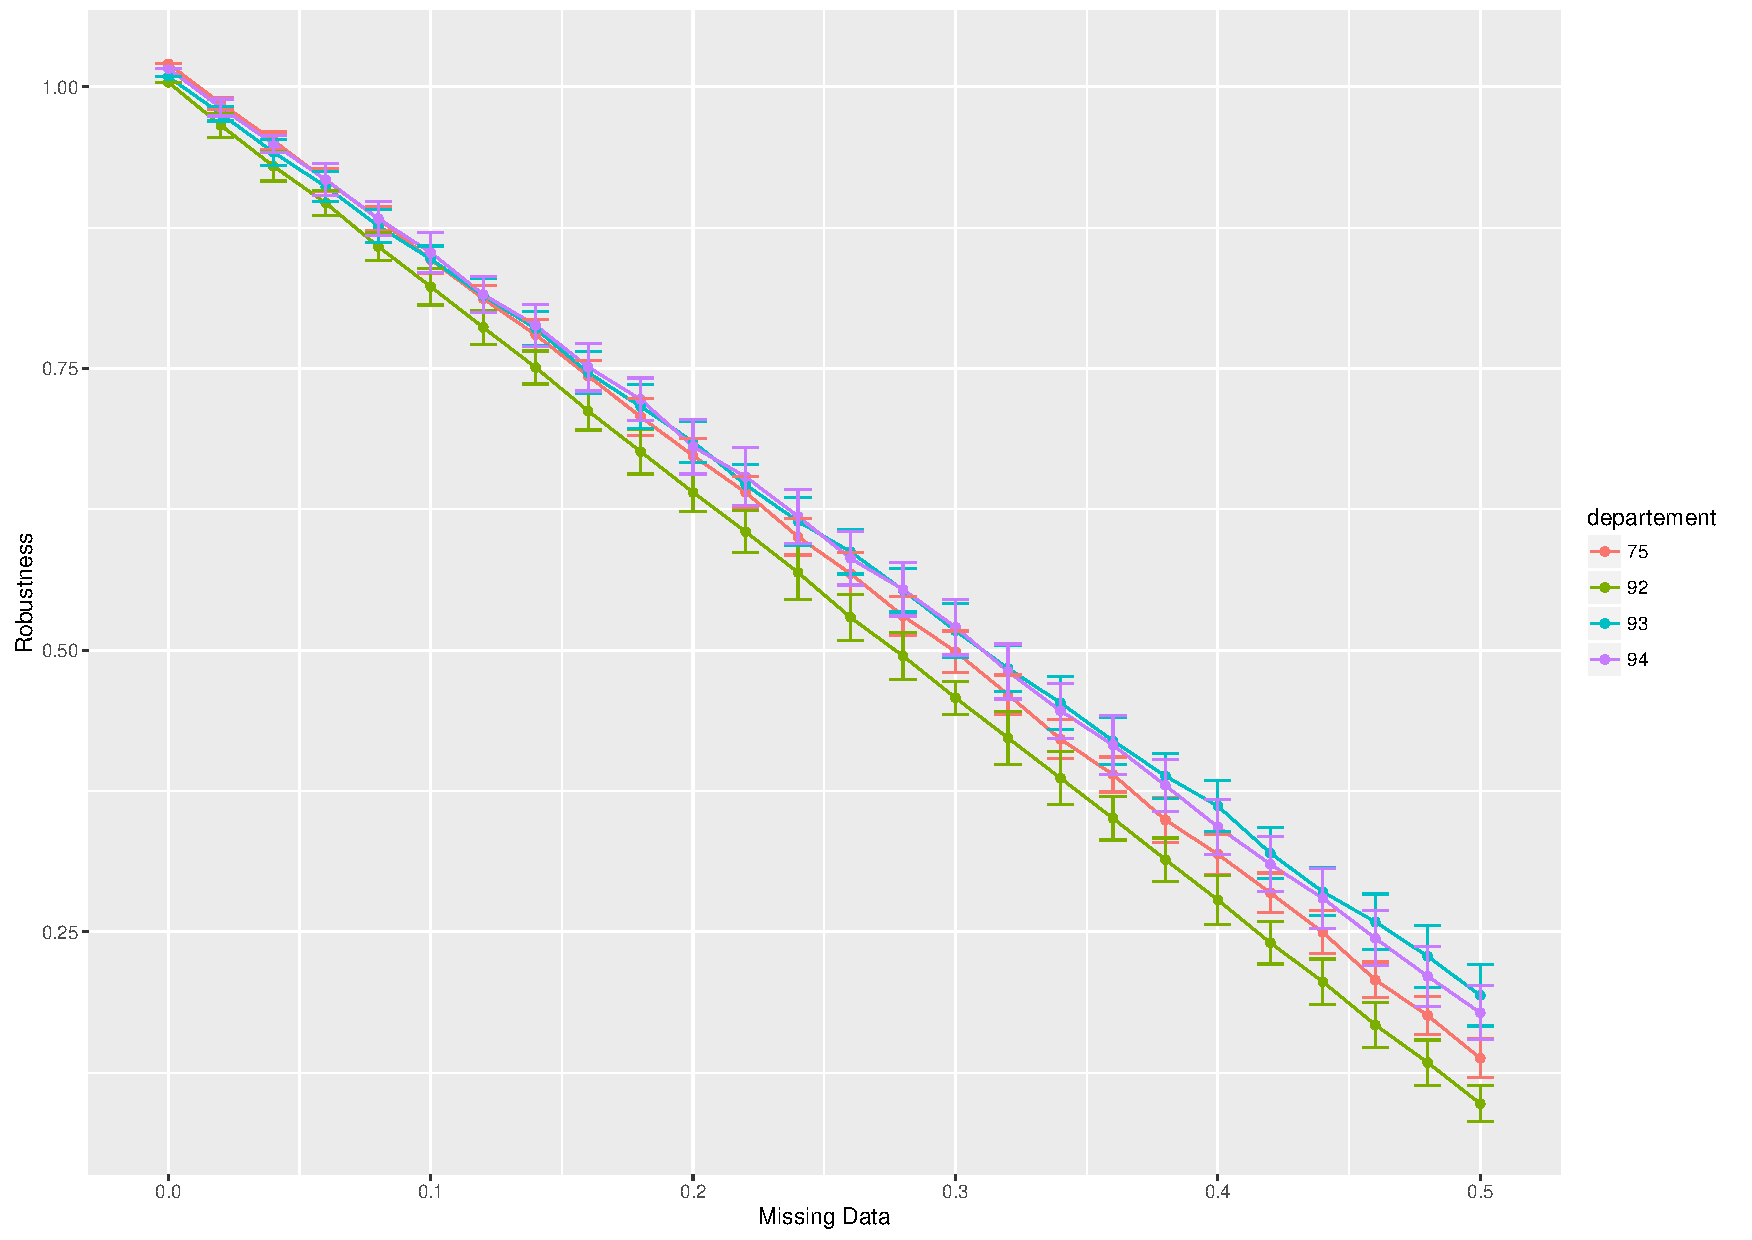
\includegraphics[width=0.7\textwidth]{figures/rob_alldeps_rob_renormindics}\\
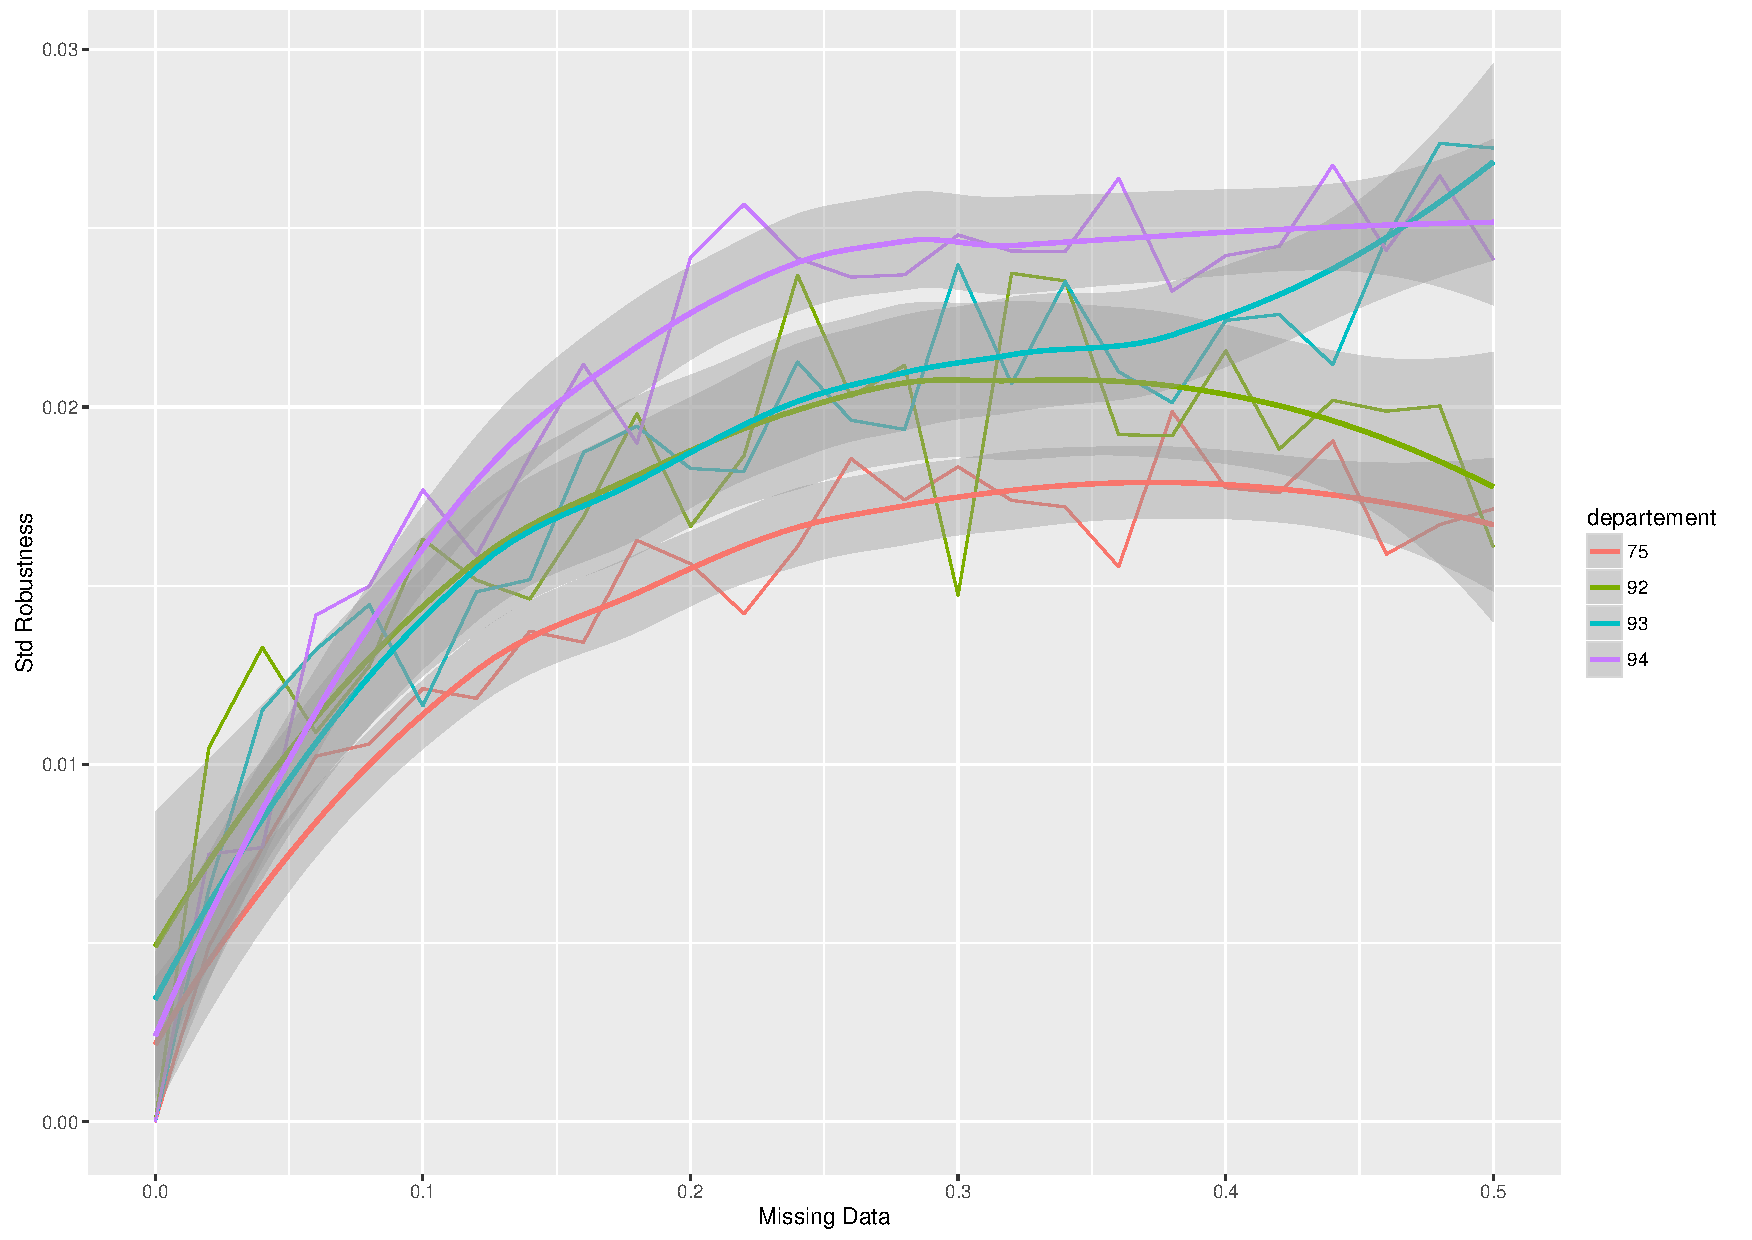
\includegraphics[width=0.7\textwidth]{figures/rob_alldeps_robsd_renormindics}


\end{columns}

}












\sframe{Meso-scale Coupled Growth}{

% RBD model : reproduces some typical urban forms

Simple co-evolutionary dynamics produce stylized urban forms at a mesoscopic scale~\cite{raimbault2014hybrid}

\bigskip
\bigskip

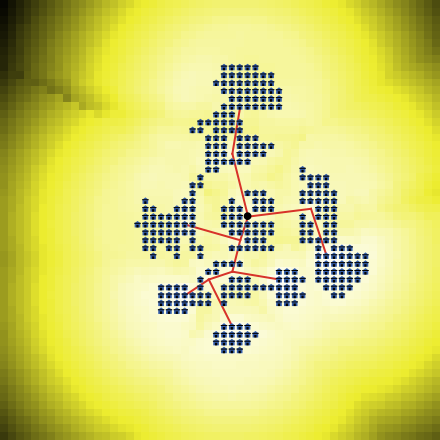
\includegraphics[width=0.3\textwidth]{figures/RBD_lattice}
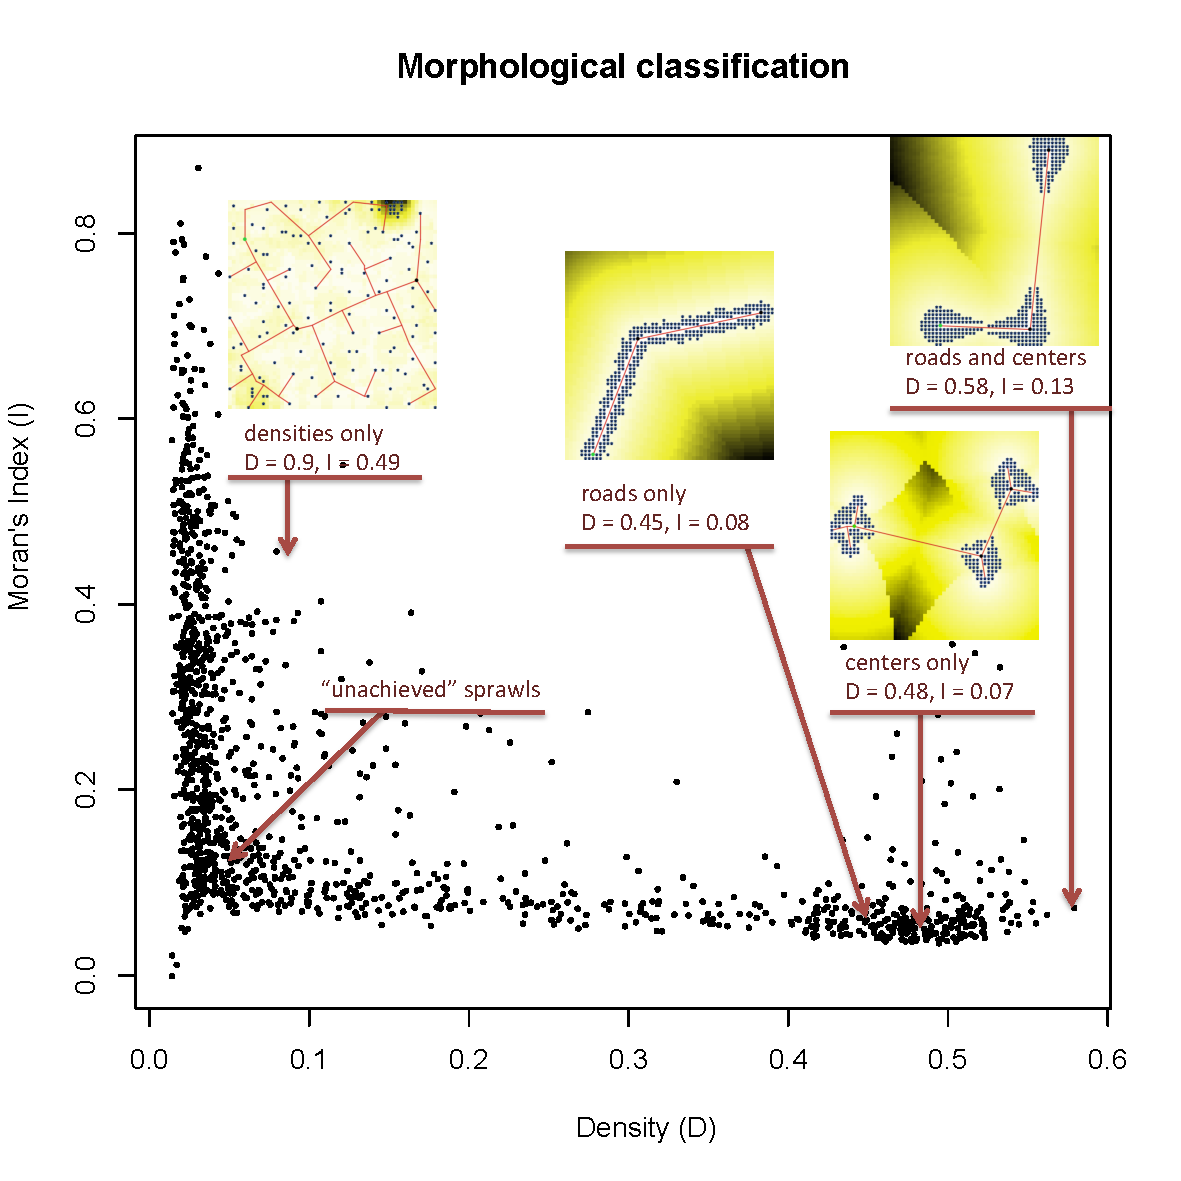
\includegraphics[width=0.35\textwidth]{figures/RBD_morpho}
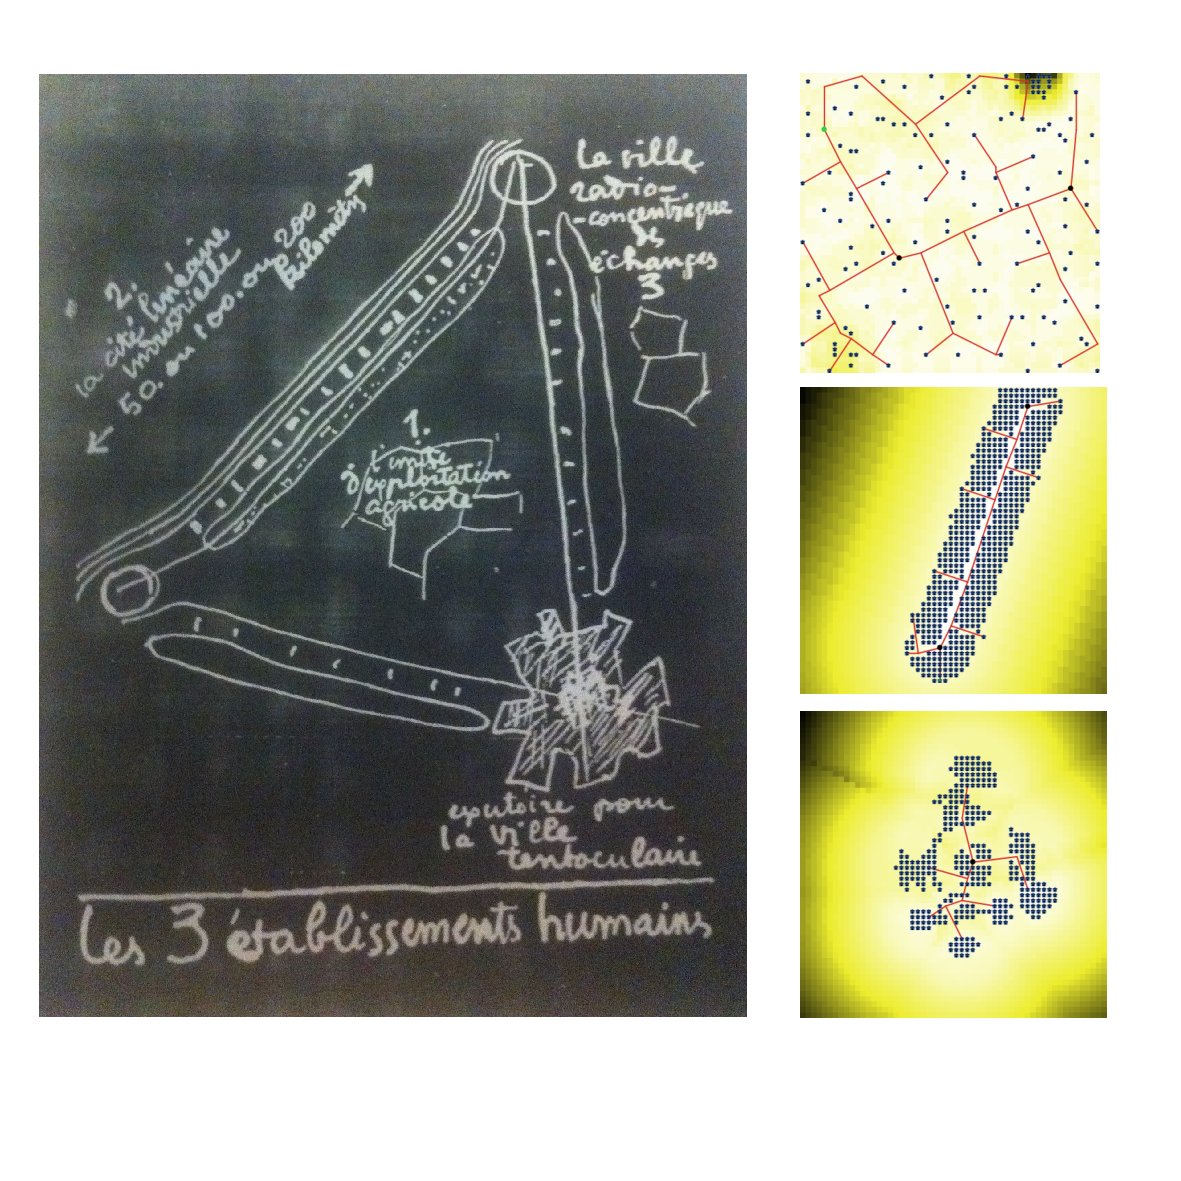
\includegraphics[width=0.35\textwidth]{figures/RBD_corbu}



}





\sframe{Transportation Network Morphogenesis}{

Transportation network morphogenesis and optimal design using biologically inspired model (slime mold) \cite{raimbault2015labex}

\bigskip

\begin{columns}
\column{0.55\textwidth}
\centering
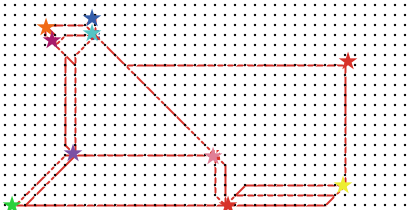
\includegraphics[width=0.9\textwidth]{figures/nwmorph_networkDense.png}

\column{0.45\textwidth}
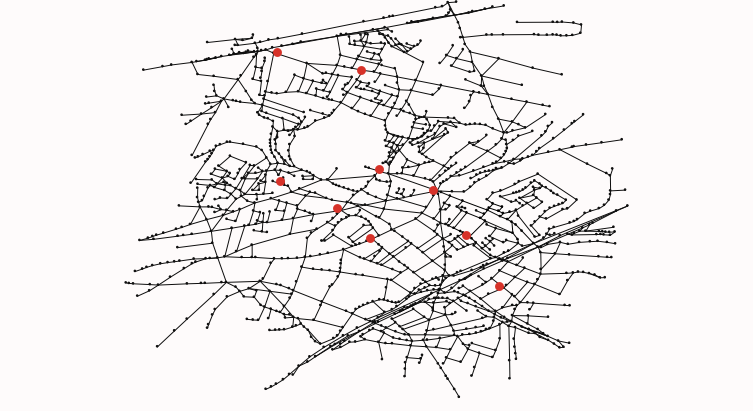
\includegraphics[width=\textwidth]{figures/nwmorph_tick1}\\
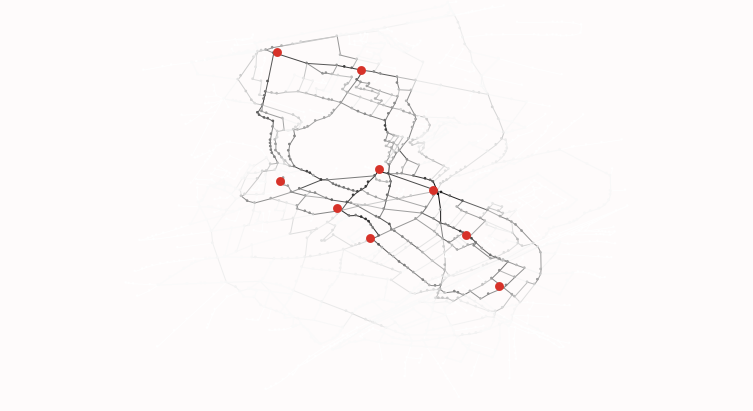
\includegraphics[width=\textwidth]{figures/nwmorph_tick101}


\end{columns}

}






\sframe{Aggregation-diffusion Urban Growth}{

% Density model

{\small Evidence of autonomous Morphogenetic processes : morphological calibration of an Aggregation-diffusion growth model}

\smallskip

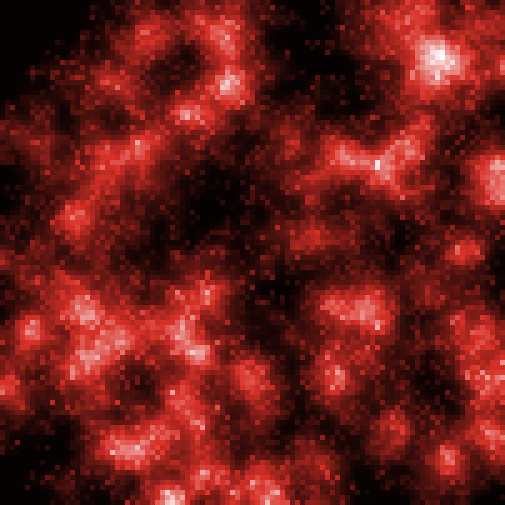
\includegraphics[width=0.24\textwidth]{figures/density_conf1}\hspace{0.1em}
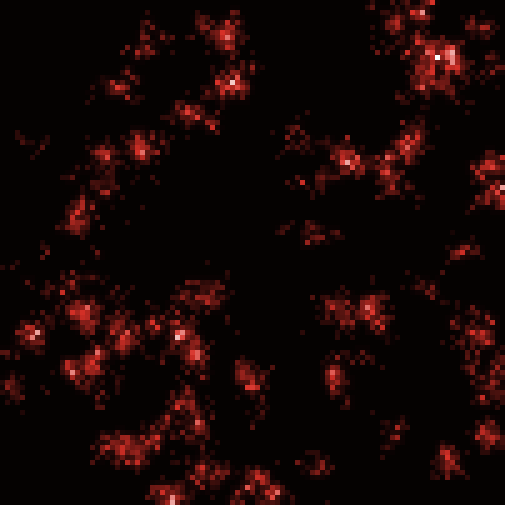
\includegraphics[width=0.24\textwidth]{figures/density_conf2}\hspace{0.1em}
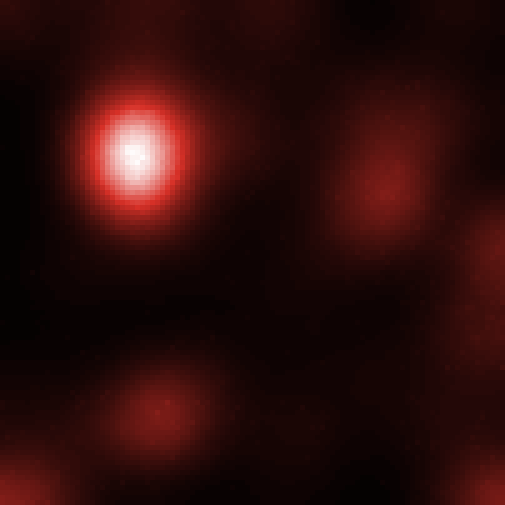
\includegraphics[width=0.24\textwidth]{figures/density_conf3}\hspace{0.1em}
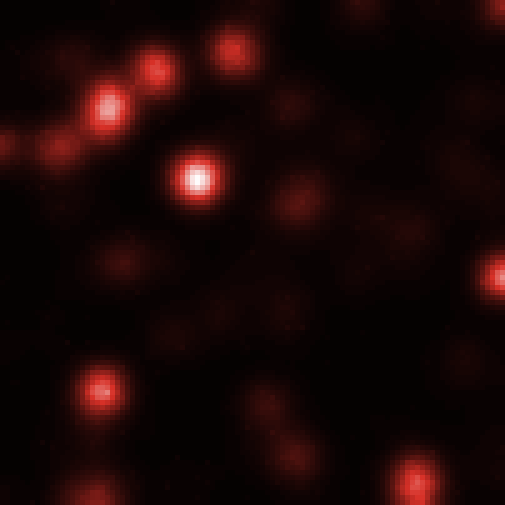
\includegraphics[width=0.24\textwidth]{figures/density_conf4}\hspace{0.1em}
\\
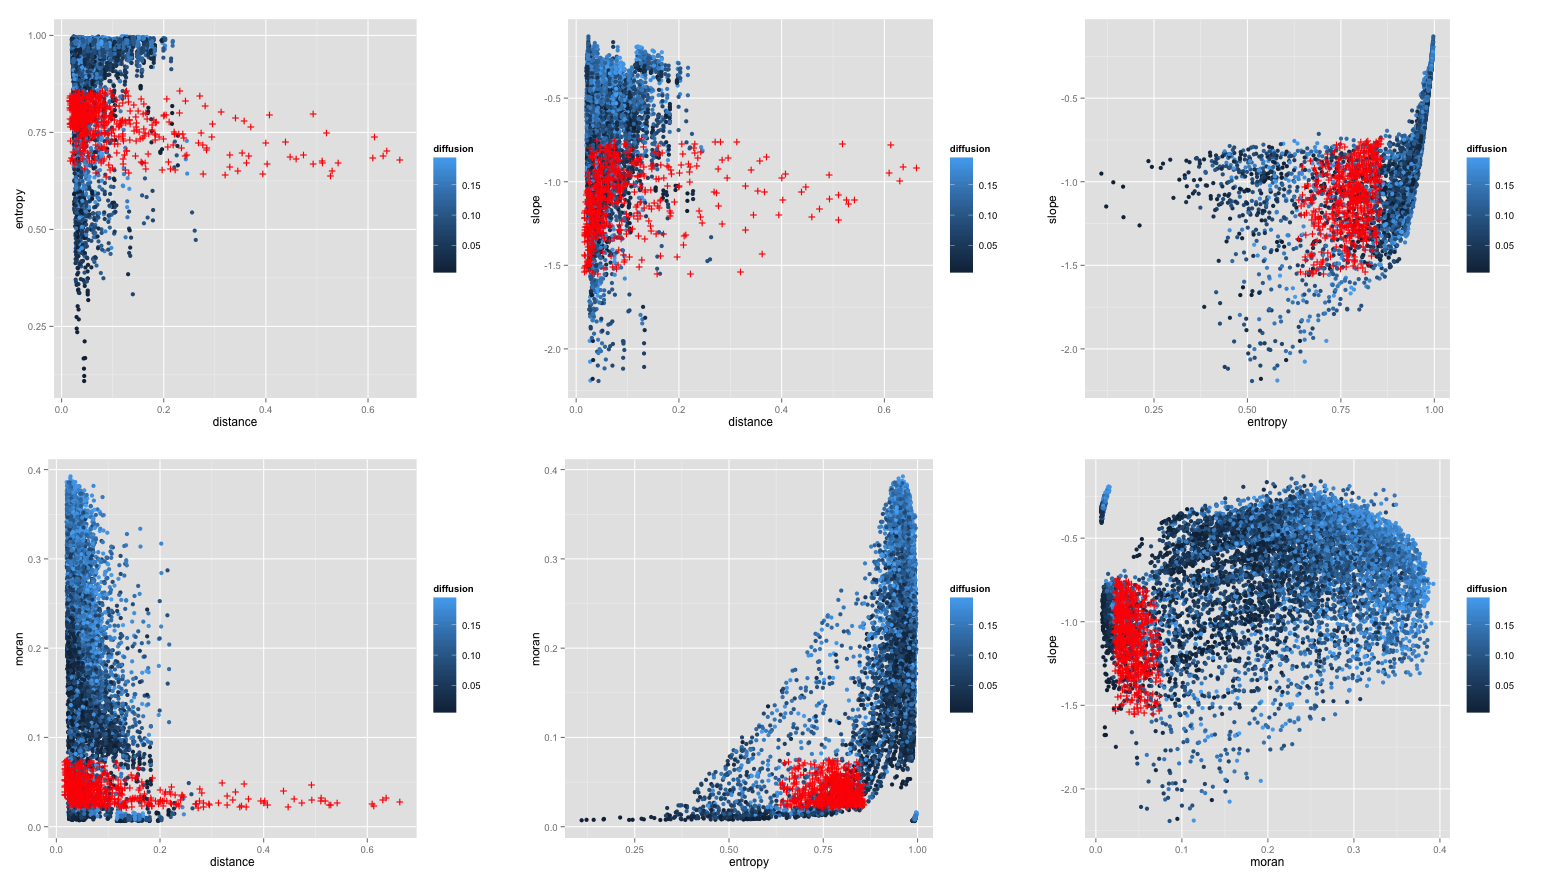
\includegraphics[width=0.5\textwidth,height=0.4\textheight]{figures/density_scatt}
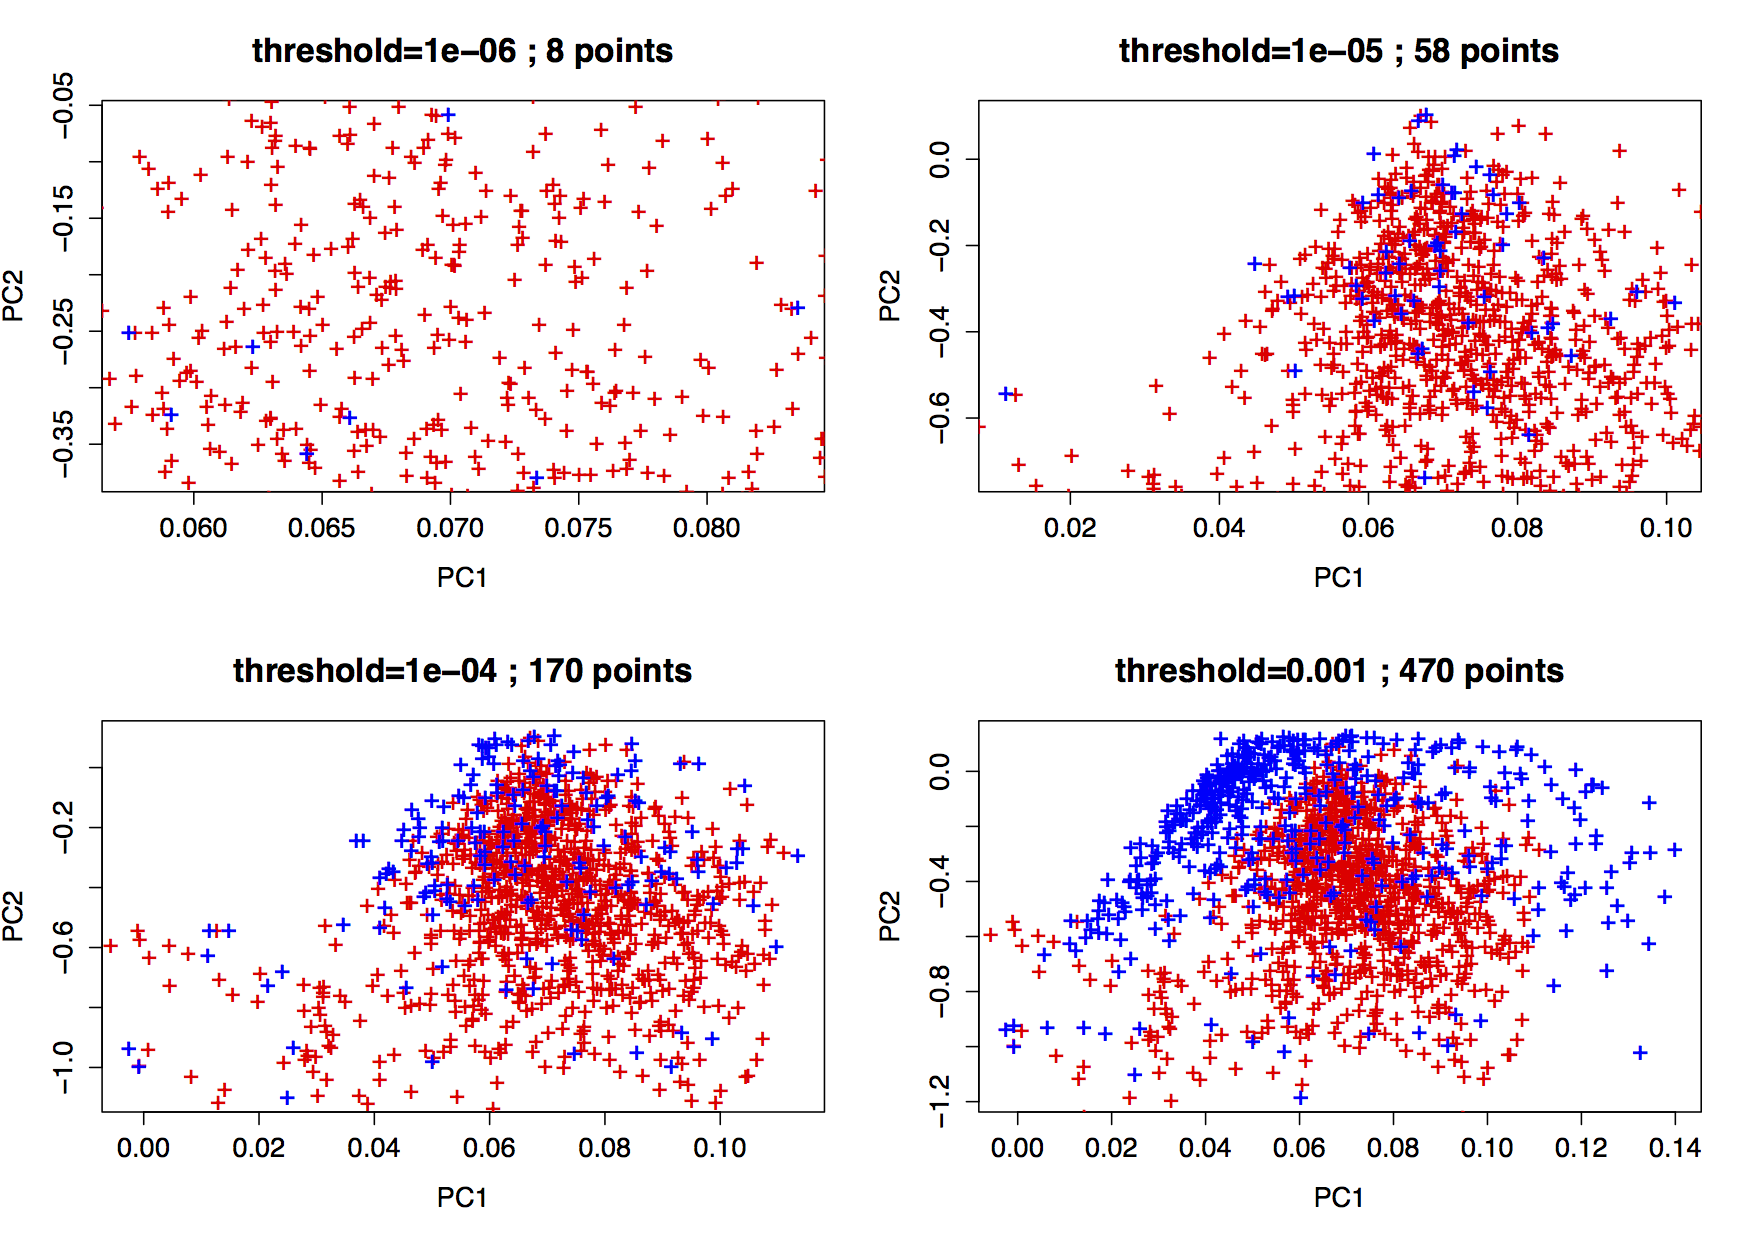
\includegraphics[width=0.5\textwidth,height=0.4\textheight]{figures/density_pca}




}


\sframe{Coupled Growth and Correlations}{

Spatial non-stationarity of correlation matrix between urban morphology and network topology~\cite{raimbault2016cautious} ; coupled growth model yield a large range of potential correlations~\cite{raimbault2016generation}


\begin{columns}
\column{0.6\textwidth}
\centering
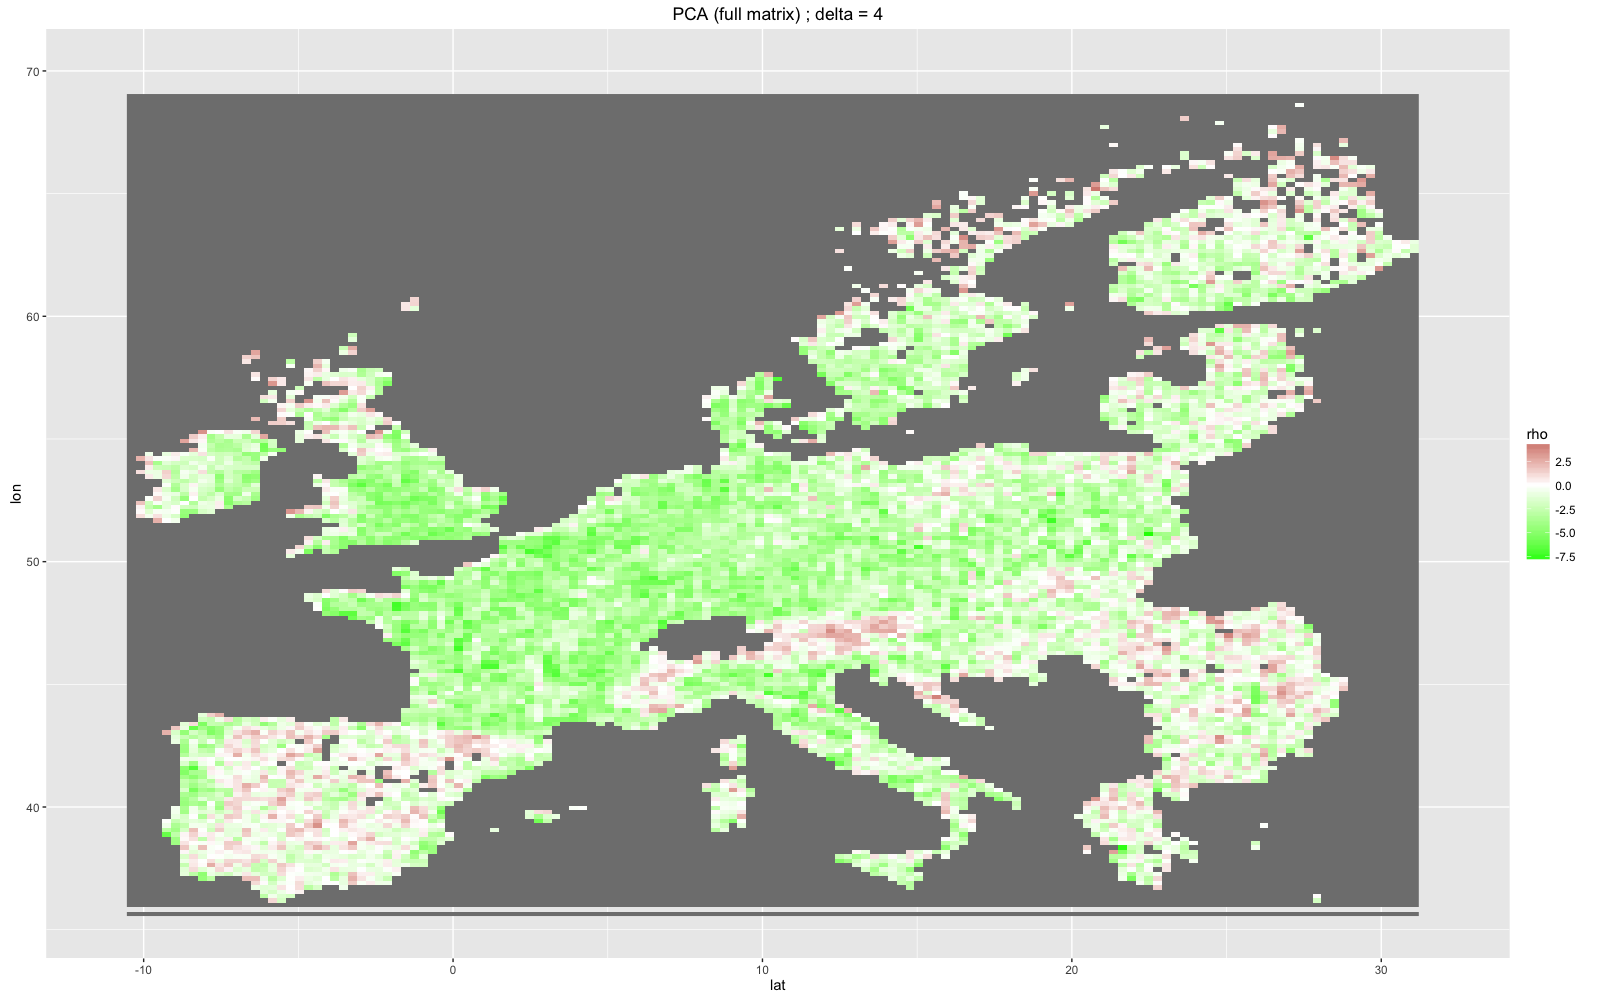
\includegraphics[width=0.65\textwidth]{figures/corr_corr_PCA_delta4}\\
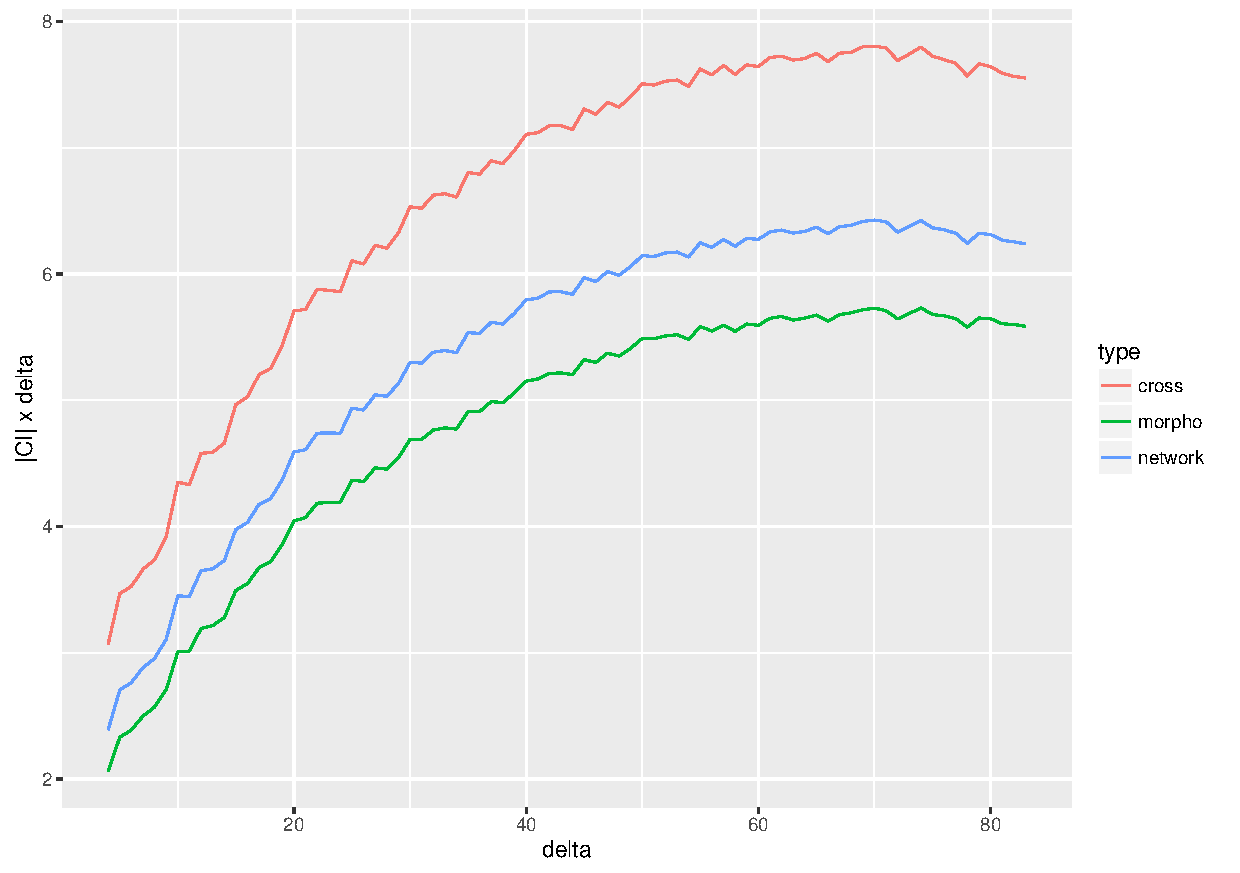
\includegraphics[width=0.65\textwidth]{figures/corr_normalized_CI_delta}

\column{0.25\textwidth}
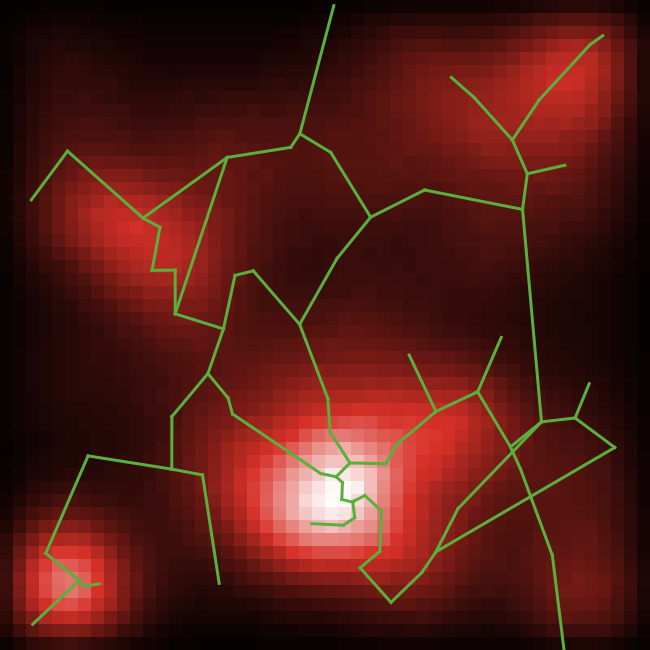
\includegraphics[width=\textwidth]{figures/corr_2_param71913_seed10}\hspace{0.1cm}\\
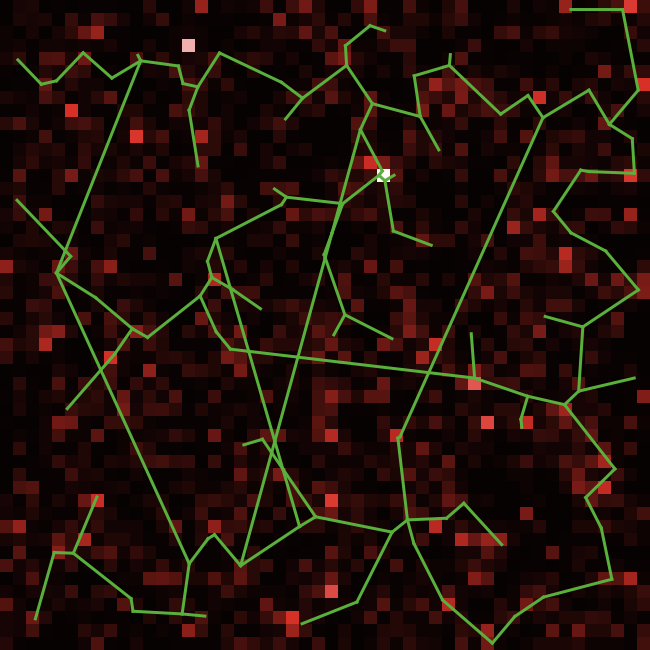
\includegraphics[width=\textwidth]{figures/corr_3_param71918_seed0}

\end{columns}

}


\sframe{Macro-scale Growth and Network Necessity}{


Macro-scale population growth model reveals physical network effects in French System of Cities~\cite{raimbault2016system}


\bigskip

\centering

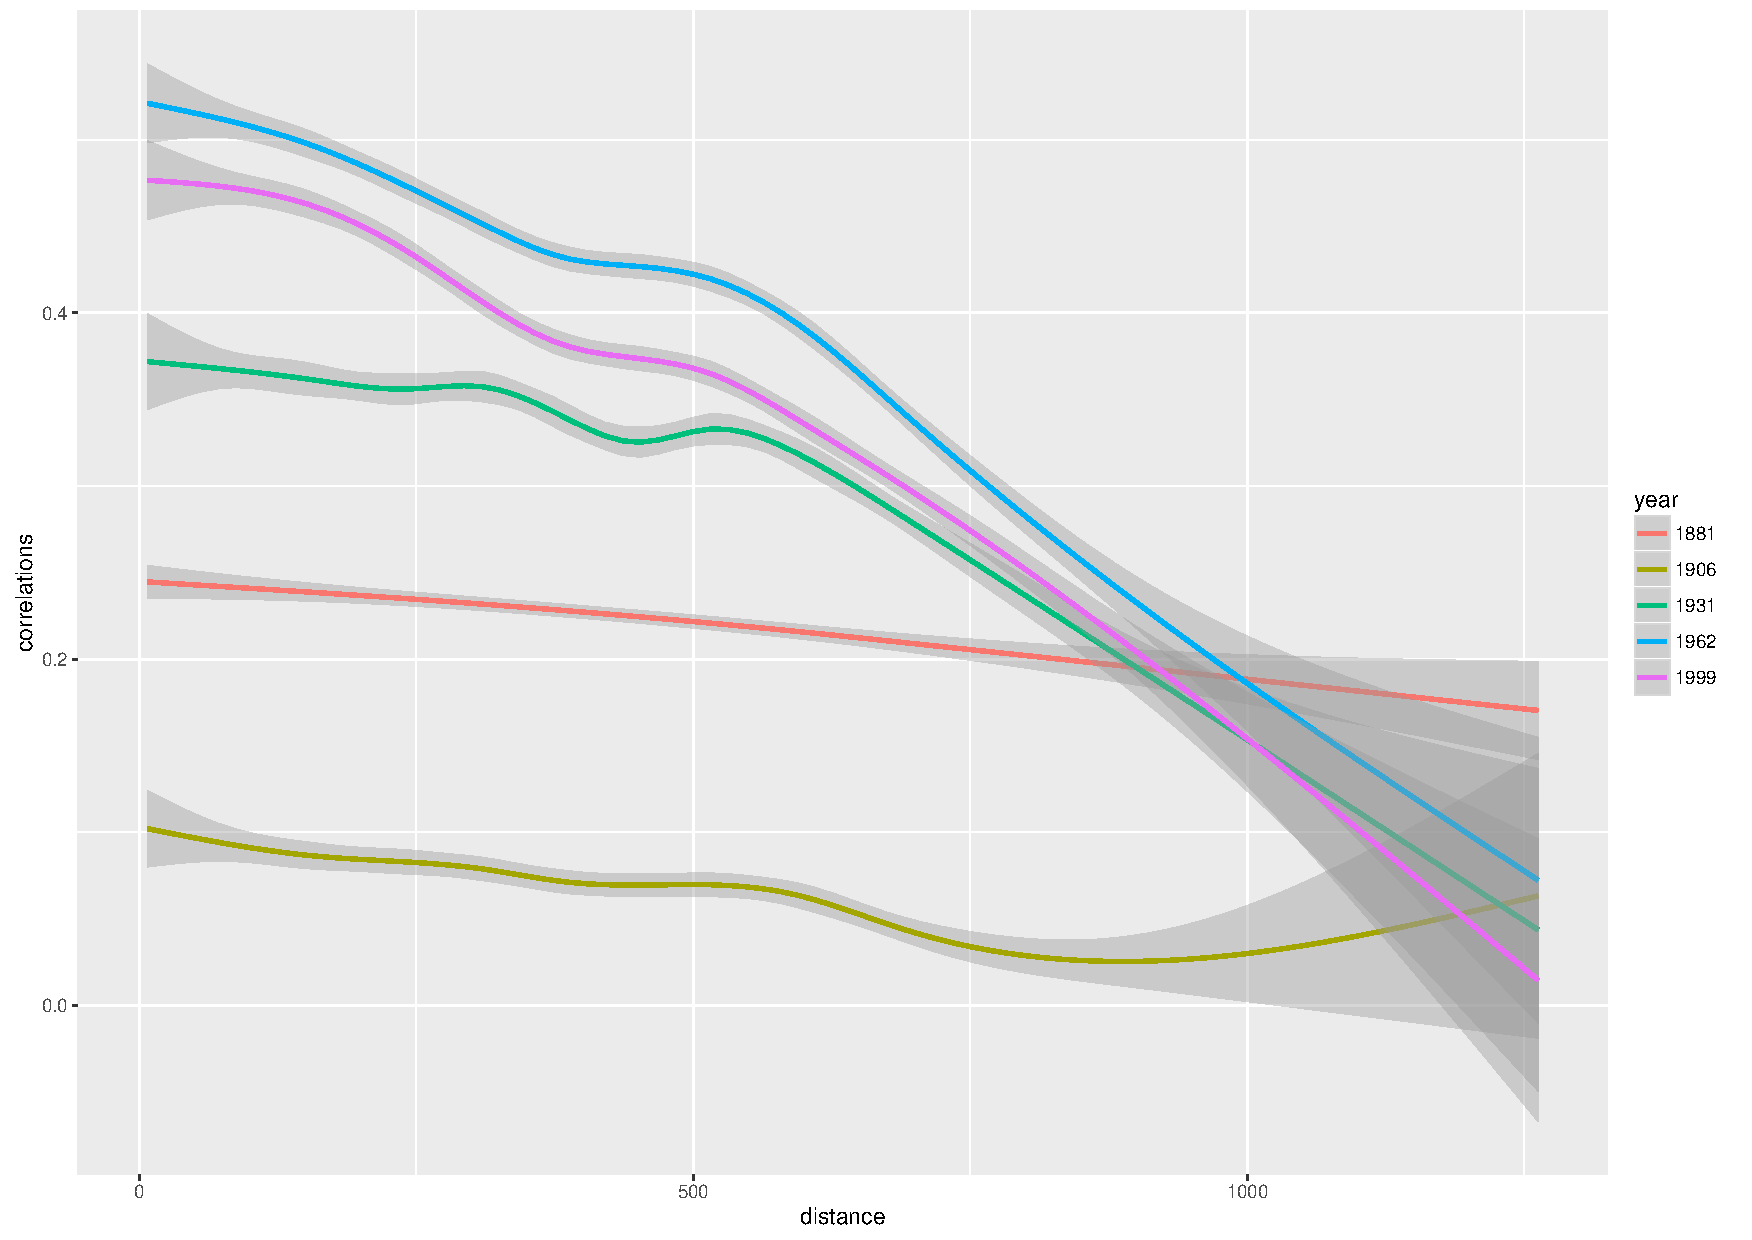
\includegraphics[width=0.3\textwidth]{figures/macro_empirical_tsCorrelations}
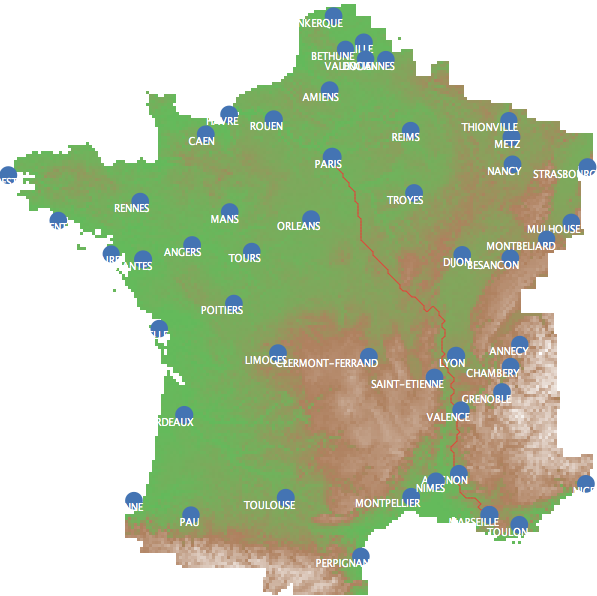
\includegraphics[width=0.3\textwidth]{figures/macro_example_shortest_path}
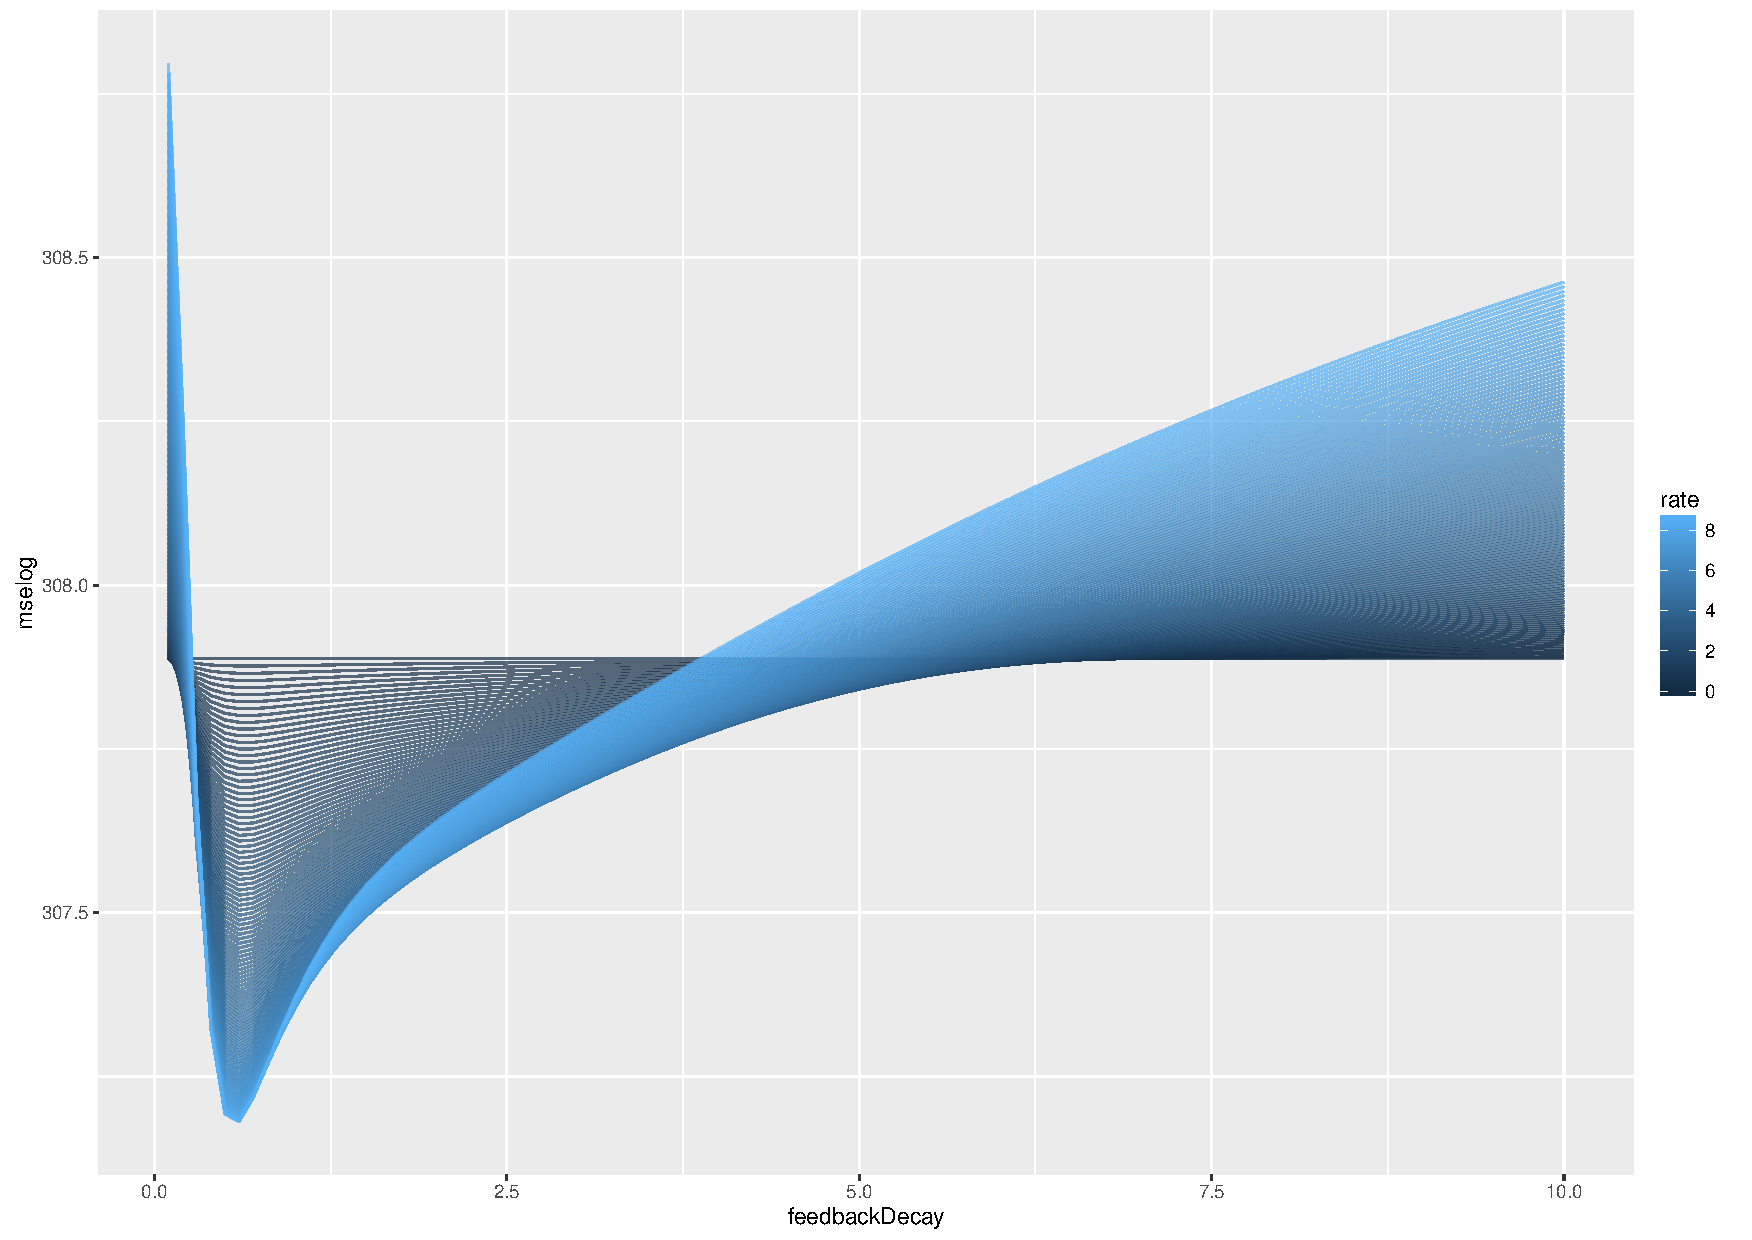
\includegraphics[width=0.3\textwidth]{figures/macro_mselog-feedbackDecay_ZOOM_fixedgravity}

}



%%%%%%%%%%%%%%%%%%%%%%%%%%%%
\sframe{Theory : Pillars}{
\begin{enumerate}
\item \textit{Networked Human Territories} $\rightarrow$ Raffestin approach to territory combined with Dupuy theory of networks.
\item \textit{Evolutive Urban Theory} $\rightarrow$ City Systems as complex Adaptive systems, applied to human settlements in general and thus territorial systems.
\item \textit{Urban Morphogenesis} $\rightarrow$ Morphogenesis as autonomous rules to explain growth of urban form. Used as the provider of modular decompositions.
\item \textit{Boundaries and Co-evolution} $\rightarrow$ Co-evolution as the existence of \textit{niche}, consequence of boundary patterns.
\end{enumerate}
}
%%%%%%%%%%%%%%%%%%%%%%%%%%%%



%%%%%%%%%%%%%%%%%%%%%%%%%%%%
\sframe{Theory : Specification}{

\textbf{Definition : } Territorial systems are networked Human Territories. They are multi-level complex adaptive systems following Evolutive Urban Theory.

\bigskip
\bigskip
\bigskip


\textbf{Hypothesis : } The existence of Morphogenetic processes in which networks are essential drivers is equivalent to the existence of co-evolutive niches in territorial systems. We call thus these \emph{Co-evolutive Networked Territorial Systems}.

}
%%%%%%%%%%%%%%%%%%%%%%%%%%%%




%\sframe{Perspective within a meta-theory ?}{
%
%Work in progress 
%
%  -> action de groupe etc. ? reflechir et garder ça pour plus tard.
%
%}




%%%%%%%%%%%%%%%%%%%
\section{Transportation Governance}
%%%%%%%%%%%%%%%%%%%



\sframe{The LUTECIA Model : Rationale}{

\justify

\textit{Mega-city Regions~\cite{hall2006polycentric} exhibit new qualitative regimes of urban systems ?}

\bigskip

$\rightarrow$ A LUTI + infrastructure provision model (LUTECIA)

\medskip

$\rightarrow$ Coevolution transport / urbanism (LUTI model with endogeneous transport infrastructure provision)

\medskip

$\rightarrow$ Game theory framework to predict emergence of centralized decision within a polycentric region

\medskip

$\rightarrow$ Importance of accessibility at MCR scale

}



\sframe{The LUTECIA Model : Structure}{

LU : Land Use module ; T : Transport module ; EC : Evaluation of Centralized decision module ; I : Infrastructure provision module ; A : Agglomeration economies module

\medskip

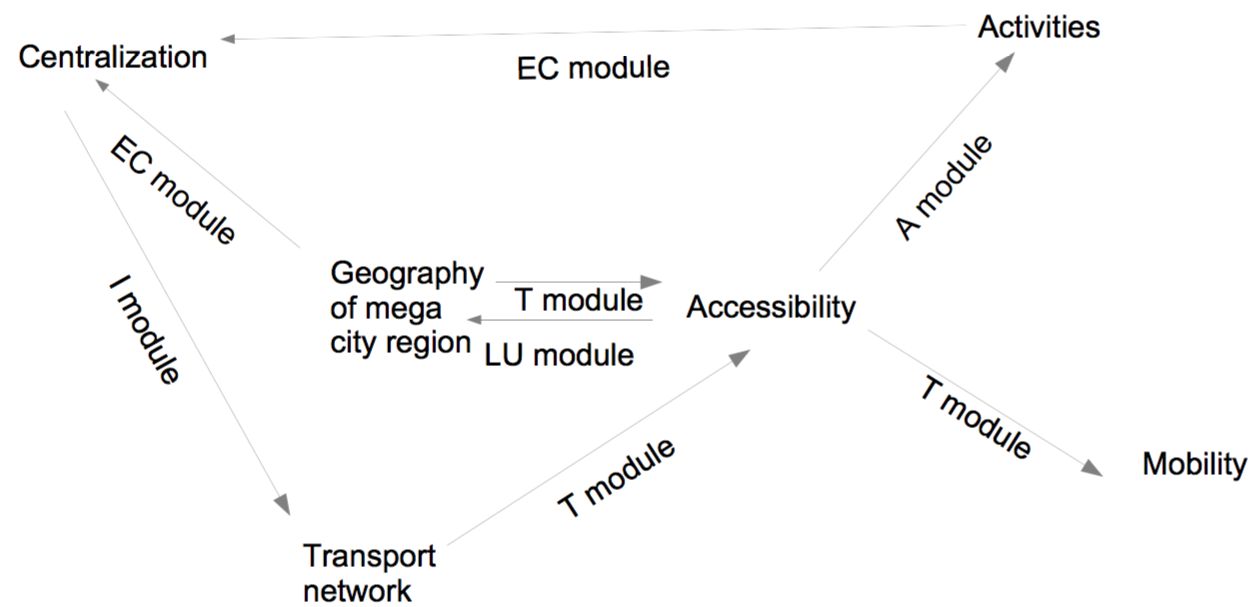
\includegraphics[width=\textwidth]{figures/lutetia_structure}

}


\sframe{Governance Modeling}{

Matrix of actors utilities, depending on respective choices

\bigskip

\begin{tabular}{ |c|c|c| } 

 \hline
 1 $|$ 2  & C & A \\ \hline
 C & $U_i = \kappa \cdot \Delta X_i(Z^{\ast}_C) - I - \frac{\delta I}{2}$
   & $\begin{cases}U_1 = \kappa \cdot \Delta X_1(Z^{\ast}_1)-I \\U_2 = \kappa \cdot \Delta X_2(Z^{\ast}_2)-I - \frac{\delta I}{2}\end{cases}$ \\ \hline
 A & $\begin{cases}U_1 = \kappa \cdot \Delta X_1(Z^{\ast}_1)-I - \frac{\delta I}{2}\\U_2 = \kappa \cdot \Delta X_2(Z^{\ast}_2)-I\end{cases}$
   & $U_i = \kappa \cdot \Delta X_i(Z^{\ast}_i) - I$ \\
 \hline
\end{tabular}


\bigskip

Two types of games implemented :
\begin{itemize}
\item Mixed Nash equilibrium, where actors compete
\item One Rational Discrete Choice equilibrium
\end{itemize}


}



\sframe{Model Output : Examples}{

\textbf{Implementation :} Netlogo ; particular treatment for dynamical programming computation of network shortest distances. Exploration with High Performance Computing on grid with \texttt{OpenMole}~\cite{reuillon2013openmole}

\medskip

\centering

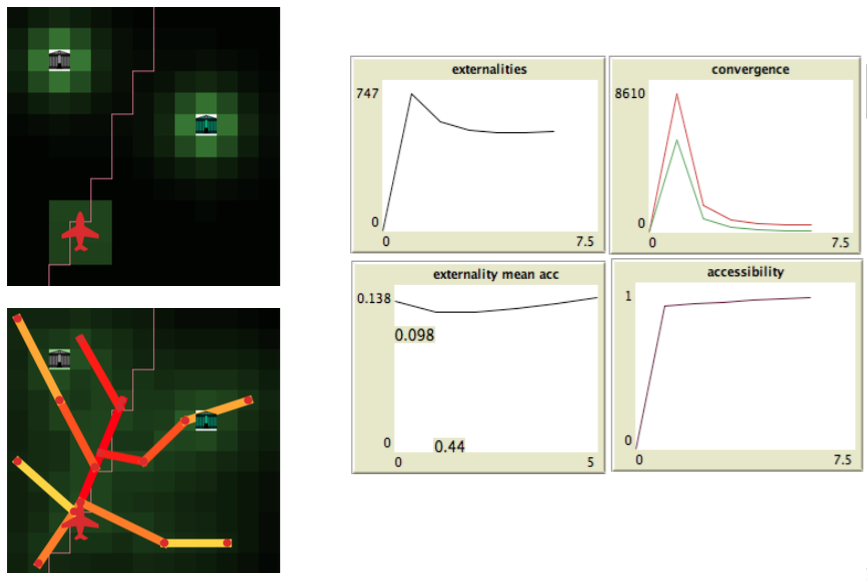
\includegraphics[width=\textwidth,height=0.7\textheight]{figures/lutetia_exrun}

}



\sframe{Model Exploration : Examples}{

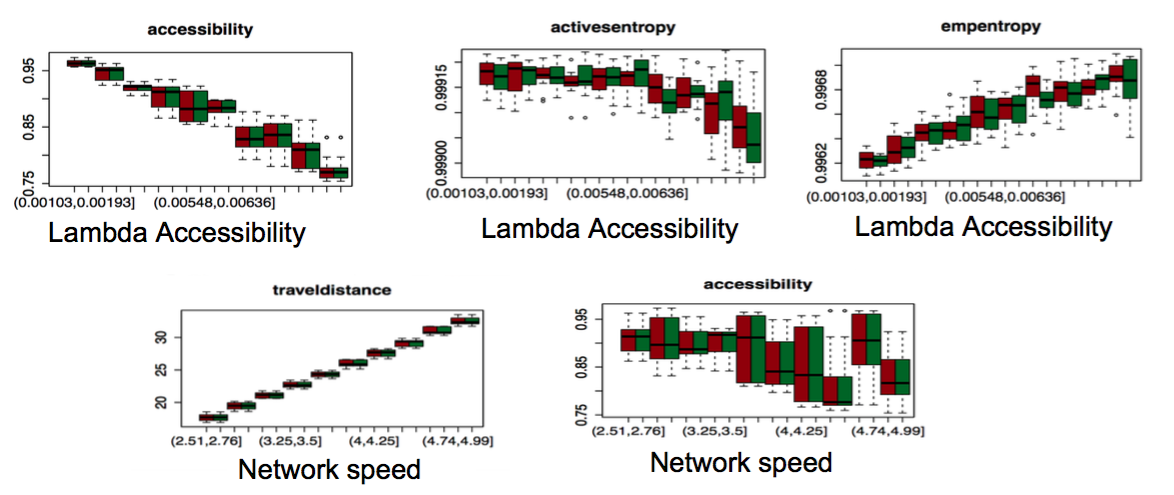
\includegraphics[width=\textwidth]{figures/lutetia_exploration}

}


\sframe{Long Time Limits for Transportation Networks}{

\centering

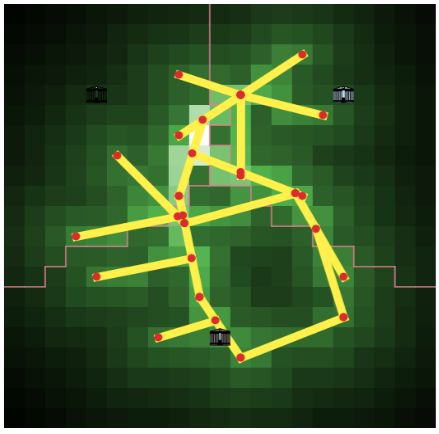
\includegraphics[width=0.4\textwidth]{figures/lutetia_longtimelimit_1}
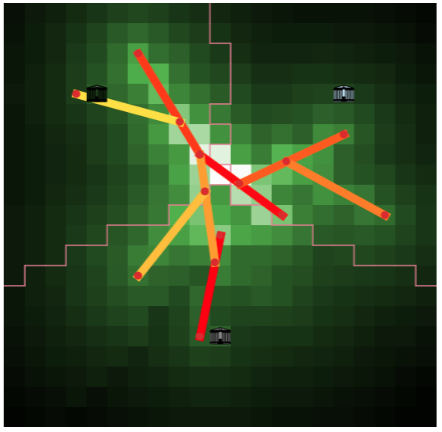
\includegraphics[width=0.4\textwidth]{figures/lutetia_longtimelimit_2}

}





\sframe{Application to Pearl River Delta Mega-city Region}{

% detail points making it a very relevant case study

Stylized characteristics of Pearl River Delta make a perfect candidate for model application

\medskip

\centering

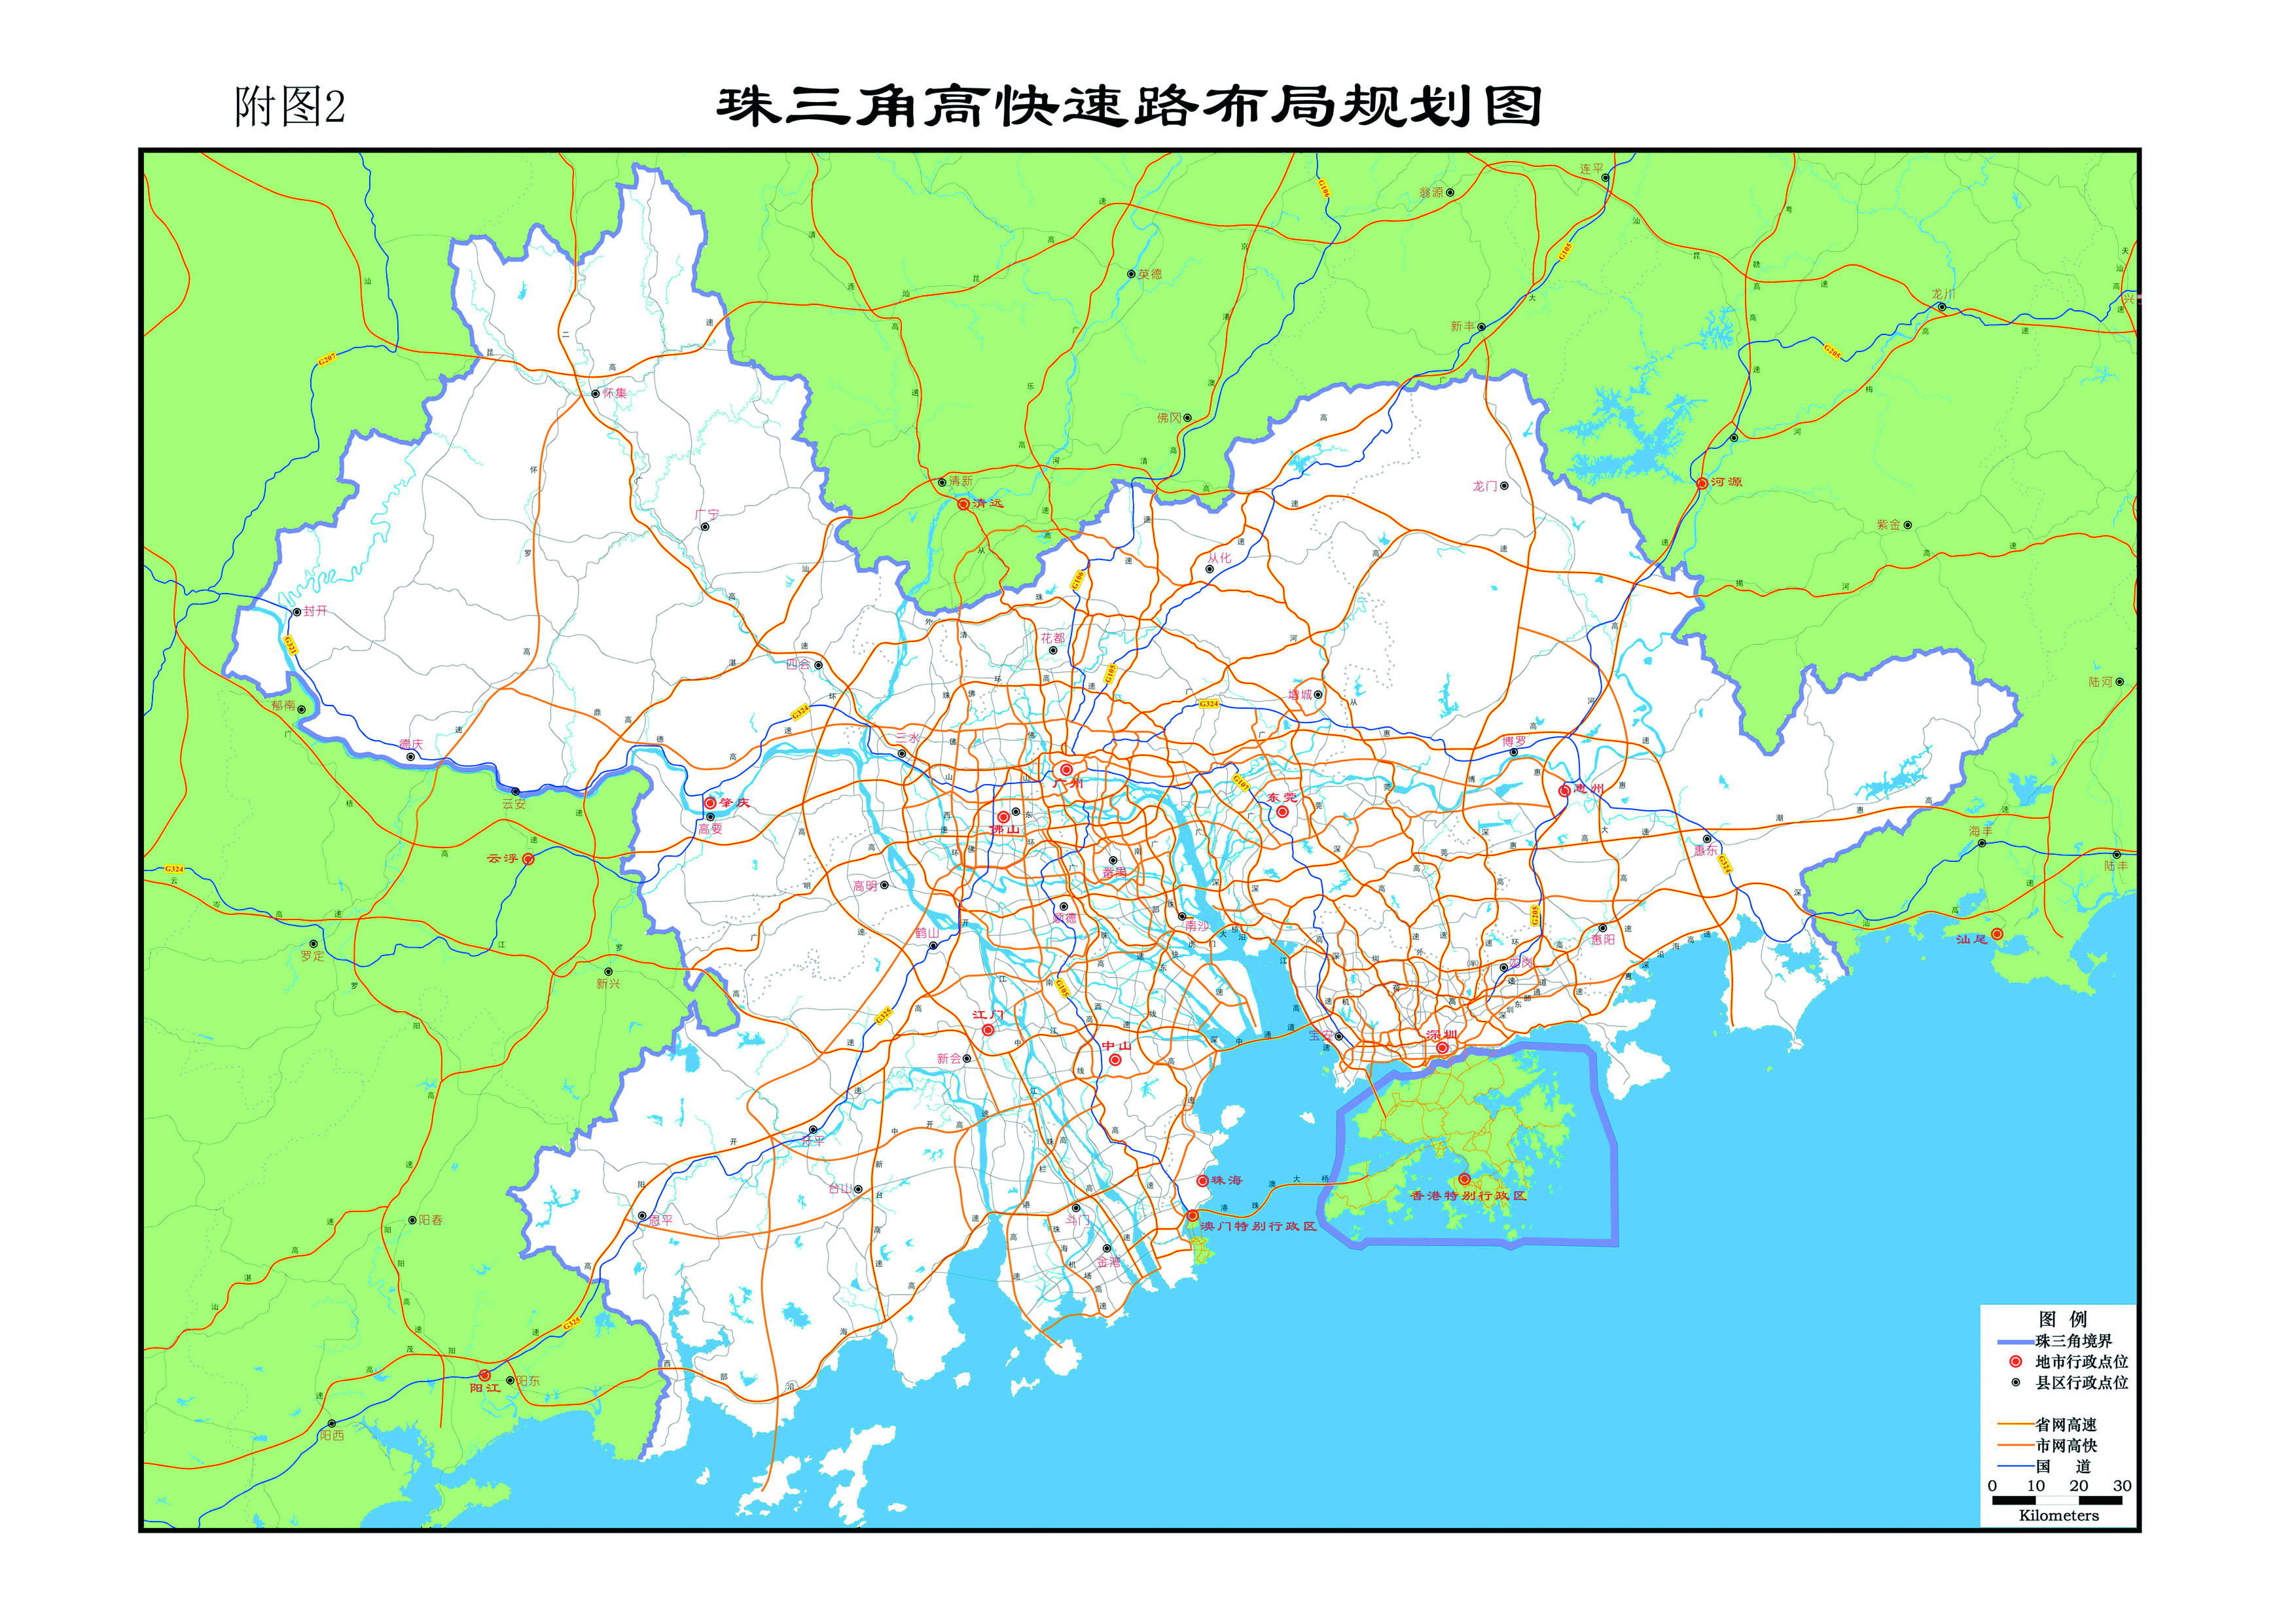
\includegraphics[width=0.6\textwidth]{figures/guangdong_masterplan}

{\tiny Source : Guangdong Province Government}

}


\sframe{Application to Pearl River Delta}{

% stylized configuration ?
%  -> requires gis import

\textbf{Specific characteristics :}

\medskip

\begin{itemize}
\item Regional Governance new level of State action ; Mega-city region roughly at regional scale.
\item Large development of infrastructures in a relatively short time
\item Local and Regional Transportation masterplans at different dates
\item Bridges across the delta : expensive infrastructure, require difficult collaboration
\item High economic competition between cities ; particular role of Hong-Kong and Macao
\end{itemize}


}




\sframe{Application : Experience plan and Expected Results}{

% still data collection, formatting, model adjustments
% network and land-use data

\textbf{Requirements : }
\begin{itemize}
\item Thematic model adaptation
\item Technical model adjustments
\end{itemize}

\medskip

\textbf{Experience plan : }
\begin{itemize}
\item Conditions for emergence of the functional MCR
\item Calibrate model retrospectively : unveil governance processes
\item Calibrate model on planned infrastructure : collaboration patterns equivalent to a central planning
\item Calibrate model on optimal infrastructure (multi-objectives to be determined) : what are corresponding "optimal" governance structures ?
\end{itemize}



}






\sframe{Conclusion}{

$\rightarrow$ From this particular model and the case study, theory should be confirmed/informed/refined/etc. (ex. : network plays indeed a crucial role in governance bifurcations, territorial systems should include explicit agents, etc. )


\medskip

$\rightarrow$ Knowledge production process is itself a metaphor of studied geographical processes : co-evolutive and complex.

\medskip

$\rightarrow$ Vertical and Horizontal integration : Interdisciplinarity beyond qualitative/quantitative artificial distinctions 


\bigskip
\bigskip
\bigskip


\footnotesize{ - All code and data available at \texttt{https://github.com/JusteRaimbault/CityNetwork/tree/master/Models}

}

}




\sframe{Reserve slides}{

\centering

\Large

\textbf{Reserve Slides}

}







\sframe{Governance Game Specification}{

Mixed Nash equilibrium probability :

\[
p_i = \frac{J}{\Delta X_{\bar{i}}{Z^{\star}_{C}} - \Delta X_{\bar{i}}{Z^{\star}_{\bar{i}}}}
\]

\medskip


% Discrete choices model

Discrete Choice model :

\[
U_i(C) - U_i(NC) = p_{\bar{i}} \left( \Delta X_{i}{Z^{\star}_{C}} - \Delta X_{i}{Z^{\star}_{i}}\right) - J
\]

then

\[
p_i = \frac{1}{1 + \exp{\left(-\beta_{DC}\cdot \left(\frac{\Delta X_{i}{Z^{\star}_{C}} - \Delta X_{i}{Z^{\star}_{i}}}{1 + \exp{\left(- \beta_{DC}(p_i \cdot (\Delta X_{\bar{i}}{Z^{\star}_{C}} - \Delta X_{\bar{i}}{Z^{\star}_{\bar{i}}}) - J)\right)}} - J \right)\right)}}
\]




}


\sframe{Lutetia : default parameter values}{

% default param values
$A_{max} = E_{max} = 500 ; r_A = 1 ; r_E = 0.8 ; \gamma_E = 0.9 ; \gamma_A = 0.65 ; \beta_{l} = 1.8 ; \lambda = 0.005 ; r_0 = 2$

$N_{expl} = 25 ; I = 0.001 ; J = 0.0001 ; \nu = 5 ; E_{ext}(t_0) = 3E_{max} ; t_f = 4$


}


\sframe{Lutetia : Land-use Initialization}{

Initial distribution of Actives and Employments around governance centers at positions $\vec{x}_i$ by
\[
A(\vec{x}) = A_{max} \cdot \exp{\left(\frac{\norm{\vec{x}-\vec{x}_i}}{r_A}\right)} ; 
E(\vec{x}) = E_{max} \cdot \exp{\left(\frac{\norm{\vec{x}-\vec{x}_i}}{r_E}\right)}
\]

}



\sframe{Lutetia : Transportation}{


Transportation module : computation of flows $\phi_{ij}$ by solving on $p_i,q_j$ by a fixed point method (Furness algorithm), the system of gravital flows
\[
\begin{cases}
\phi_{ij} = p_i q_j A_i E_j \exp{\left(-\lambda_{tr} d_{ij}\right)}\\
\sum_k \phi_{kj} = E_j ; \sum_k \phi_{ik} = A_i\\
p_i = \frac{1}{\sum_k{q_k E_k \exp{(-\lambda_{tr}d_{ik})}}} ; q_j = \frac{1}{\sum_k{p_k A_k \exp{(-\lambda_{tr}d_{kj})}}} 
\end{cases}
\]

Trajectories then attributed by effective shortest path, and corresponding congestion $c$ obtained (no Wardrop equilibrium). 

Speed of network given by BPR function $v(c) = v_0 \left(1 - \frac{c}{\kappa}\right)^{\gamma_c}$. Congestion not used in current studies (infinite capacity $\kappa$).





}



\sframe{Lutetia : Land-use Evolution}{



Land-Use module : we assume that residential/employments relocations are at equilibrium at the time scale of a tick, that corresponds to transportation infrastructure evolution time scale which is much larger (Bretagnolle, 2009).

We take a Cobb-douglas function for utilities of actives/employments at a given cell
\[
U_i (A) = X_i(A)^{\gamma_A}\cdot {F_i(A)}^{1-\gamma_A} ; F_i(A) = \frac{1}{A_i E_i}
\]
\[
U_j (E) = X_j(E)^{\gamma_E}\cdot {F_j(E)}^{1-\gamma_E} ; F_j(E) = 1
\]

where $X_i(A) = A_i\cdot \sum_j{E_j \exp{\left(-\lambda\cdot d_{ij}\right)}}$ and $X_j(E) = E_j\cdot \sum_i{A_i \exp{\left(-\lambda\cdot d_{ij}\right)}}$.

Relocations are then done deterministically following a discrete choice model :
\[
A_i(t+1) = \sum_i{A_i(t)}\cdot\frac{\exp{(\beta U_i(A))}}{\sum_i{\exp{(\beta U_i(A))}}}
\]
\[
E_j(t+1) = \sum_j{E_j(t)}\cdot\frac{\exp{(\beta U_j(E))}}{\sum_j{\exp{(\beta U_j(E))}}}
\]




}



\sframe{Lutetia : Network Distance Computation}{



Effective distances computation

\begin{itemize}
\item Euclidian distance matrix $d(i,j)$ computed analytically
\item Network shortest paths between network intersections (rasterized network) updated in a dynamic way (addition of new paths and update/change of old paths if needed when a link is added), correspondance between network patches and closest intersection also updated dynamically ; $O(N_{inters}^3)$
\item Weak component clusters and distance between clusters updated ; $O(N_{nw}^2)$
\item Network distances between network patches updated, through the heuristic of only minimal connexions between clusters ; $O(N_{nw}^2)$
\item Effective distances (taking paces/congestion into account) updated as minimum between euclidian time and $\min_{C,C'}{d(i,C)+d_{nw}(p_C(i),p_C'(j))+d(C',j)}$ ; $O(N_{clusters}^2\cdot N^2)$ [Approximed with $\min_C$ only in the implementation, consistent within the interaction ranges $\sim$ 5 patches taken in the model]. 
\end{itemize}


}

\sframe{Lutecia : Exploration}{
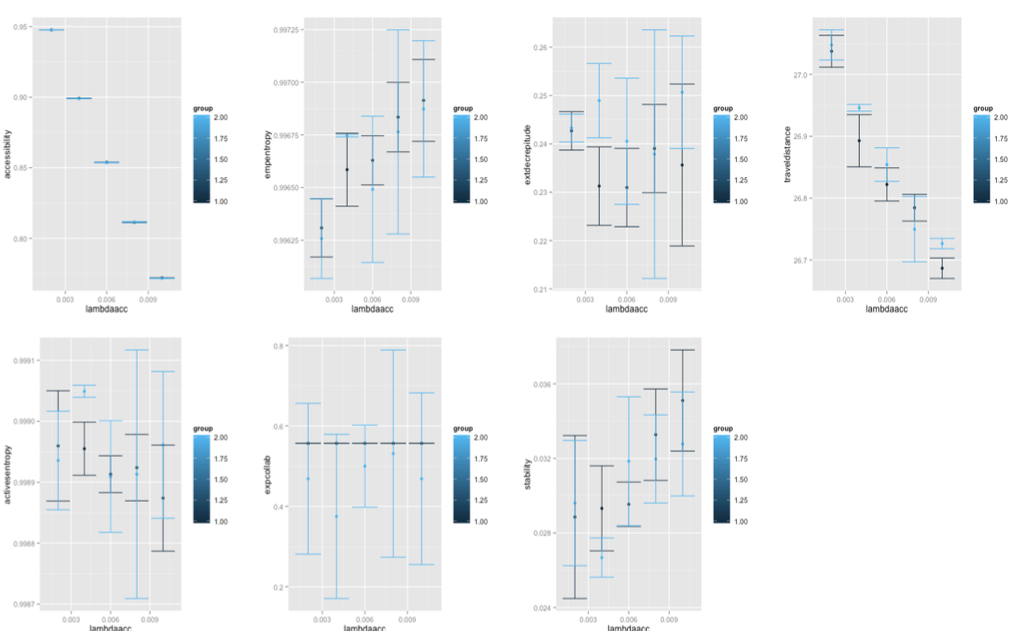
\includegraphics[width=\textwidth]{figures/lutecia_sens1}
}

\sframe{Lutecia : Exploration}{
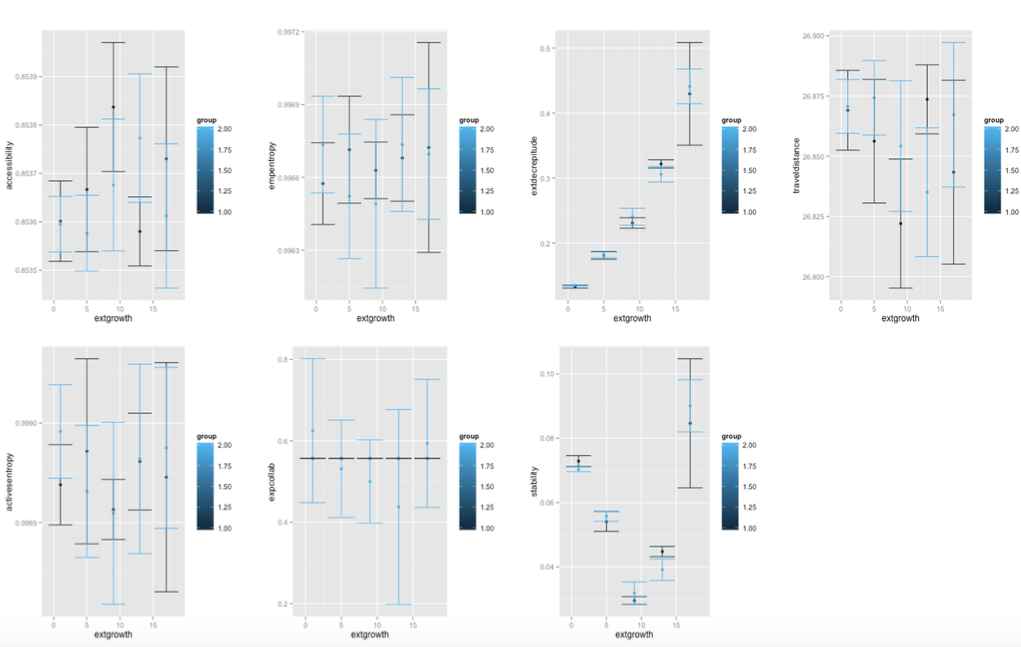
\includegraphics[width=\textwidth]{figures/lutecia_sens2}
}


\sframe{Lutecia : Exploration}{
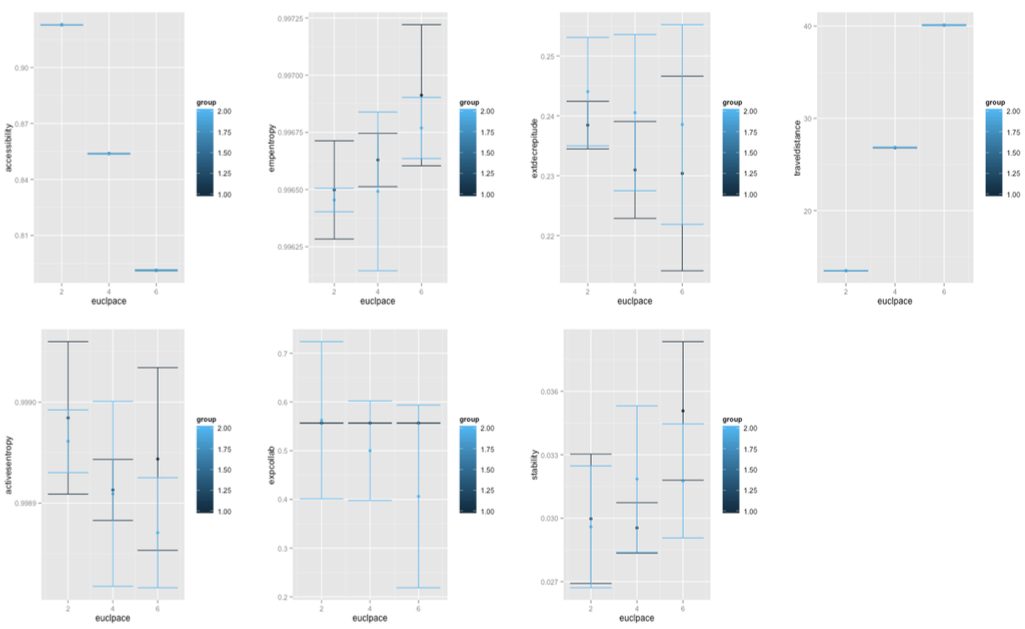
\includegraphics[width=\textwidth]{figures/lutecia_sens3}
}

\sframe{Lutecia : Exploration}{
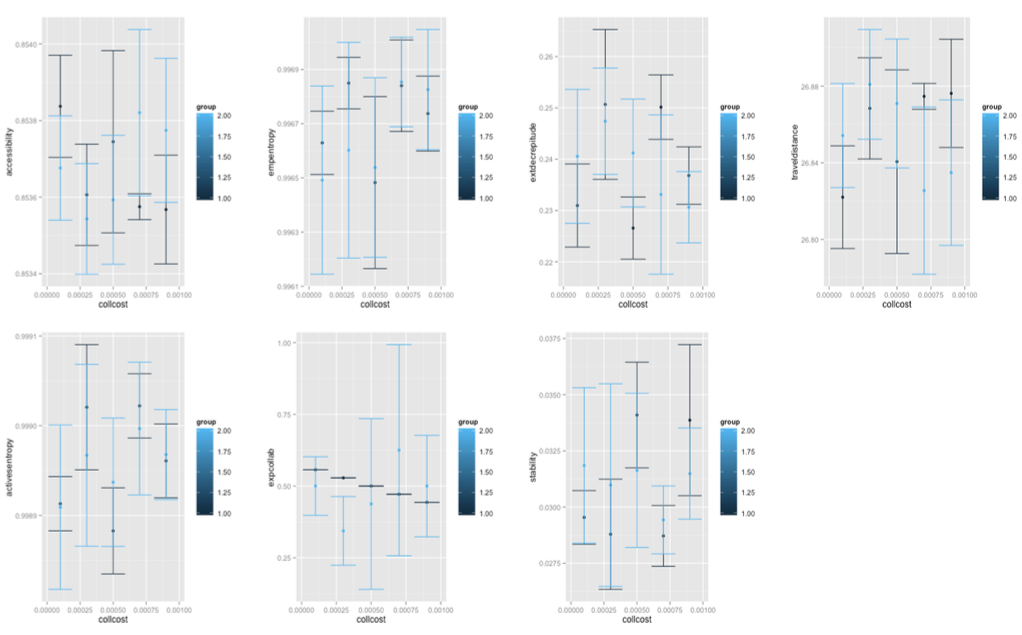
\includegraphics[width=\textwidth]{figures/lutecia_sens4}
}




%%%%%%%%%%%%%%%%%%%%%
\begin{frame}[allowframebreaks]
\frametitle{References}
\bibliographystyle{apalike}
\bibliography{/Users/Juste/Documents/ComplexSystems/CityNetwork/Biblio/Bibtex/CityNetwork,biblio}
\end{frame}
%%%%%%%%%%%%%%%%%%%%%%%%%%%%






\end{document}







